\documentclass{article}

% these packages let you do math
\usepackage{amsmath}
\usepackage{amssymb}

% we need these packages for fancy R tables
\usepackage{booktabs}
\usepackage{float}
\usepackage{colortbl}
\usepackage{xcolor}
\usepackage{longtable}
\usepackage{lscape}
\usepackage{threeparttablex}


% these packages play with the spacing/margins of the document. Uncomment the commands on lines 16 and 17 to see what they do.
\usepackage{a4wide}
\usepackage{setspace}
\usepackage{geometry}
\usepackage{parskip}
%\doublespacing
\geometry{margin=1.5in}

% this package helps us with including images. Setting the graphics path makes it easier to refer to things in the \includegraphics command.
\usepackage{graphicx}
\usepackage{subfig}
\graphicspath{ {../figures/final_figures} }
\newcommand*\InputTable[1]{\input{../tables/#1.tex}}
% make some hyperlinks using the \href command
\usepackage{hyperref}
\hypersetup{
    colorlinks=true,
    linkcolor=black,
    urlcolor=blue, 
    citecolor=blue
}

%citations
\usepackage{cite}
\usepackage{natbib}
\usepackage{apalike}

% set the author, title, and date of the document. \maketitle adds it to the document.
\author{Brandon Williams and Scott Kjorlien}
\title{Evaluating State-Level EITC Impact on Poverty and Labor with Synthetic Control}
\date{Spring 2022}

\begin{document}
\maketitle

\section{Introduction}

The Earned Income Tax Credit (EITC) is a tax credit that is designed to benefit workers earning relatively low wages. The program was created at the federal level in the 1970s with a dual purpose: encourage families in poverty to enter the workforce and reduce the tax burdens for low-wage working families with children. Since then, the EITC has been expanded and increased several times, becoming a significant anti-poverty measure. Some estimates suggest that the EITC has lifted more children out of poverty than any other government program  \citep{zahradnik2004state}. In 2020, the IRS reported that 25 million workers received over \$60 million in EITC credits, with the average amount being \$2,411 per family.\footnote{https://www.eitc.irs.gov/eitc-central/statistics-for-tax-returns-with-eitc/statistics-for-tax-returns-with-the-earned-income} The American Rescue Plan of 2021 further leveraged the EITC as a main means of fighting poverty in the wake of the COVID-19 pandemic by expanding the credit for childless workers and increasing income limits, indicating just how important it has become in the policymaker’s anti-poverty arsenal.

While much economic literature has focused on this tool at the federal level, very few papers have examined state EITCs, even though 29 states currently offer their own EITC to supplement the federal credit. We exploit two major changes to state EITCs in the last ten years: namely, the elimination of North Carolina's EITC in 2014 and the creation of California's EITC in 2015. Using a synthetic control design, we explore the state-level EITC impact on poverty rate and labor force participation. We find a modest increase in the labor force participation in the presence of a state EITC, but we find very little evidence for an effect on the overall poverty rate regardless of the creation or elimination of a state EITC. 

\section{Background}

The EITC is designed to “phase in” beginning with the first dollars a worker earns. In 2021, a married couple with two children, for example, had a phase-in rate of 45 percent, meaning that the EITC increases by 45 cents for each dollar earned. At a certain income threshold, the EITC plateaus at a maximum amount, where it stays constant even as the worker’s income increases. Finally, it reaches a “phase out” period, where the EITC amount reduces as a percentage of the worker’s income until it eventually reaches zero. In 2021, this phase-out ended for childless earners at \$15,820, \$42,158 for those with on child, \$47,915 for those with two children, and so on. This creates an acute trapezoid shape to the credit that increases and decreases proportionally with income. Figure~\ref{fig:tax} shows the structure of the credit based on income, with the American Rescue Plan expansion included. 

 \begin{figure}[H]
    \caption{Design of EITC}
    \begin{center}
        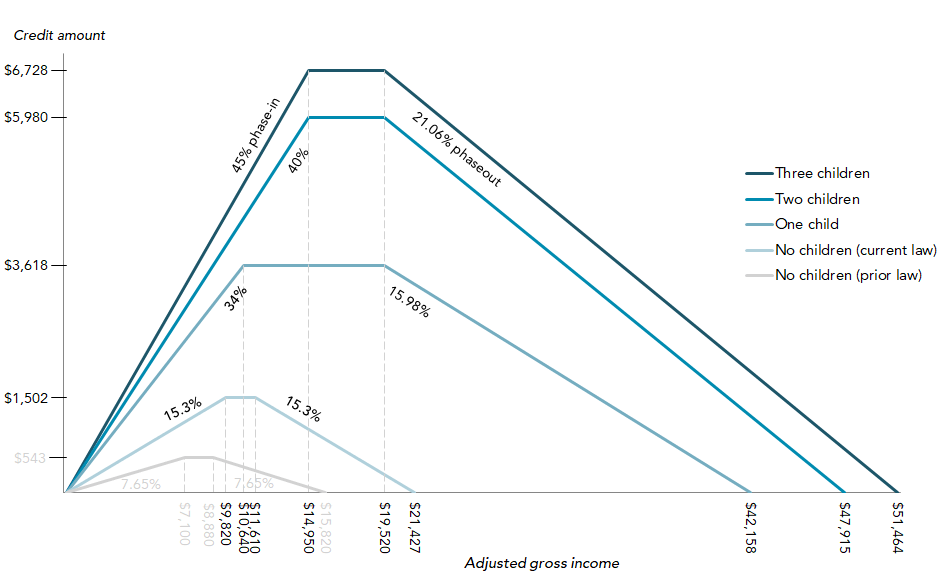
\includegraphics[width=.85\textwidth]{eitc_design}
    \end{center}
	\footnotesize
    \label{fig:tax}{Source: Tax Policy Center}
\end{figure}

Proponents of the EITC generally argue that it avoids the adverse incentives of other traditional welfare programs by encouraging workforce participation while simultaneously targeting low-income earners. Economic theory would suggest that the EITC would be especially pronounced at the point of entry for the labor supply, encouraging those on the sidelines to enter the workforce because it rewards earnings and gives no payout if the tax filer is not in the labor force \citep{eissa2006behavioral}. EITCs also avoid the mired debates about the minimum wage by increasing earnings for workers without shifting the cost to employers. In short, EITCs enjoy support from a diverse coalition of policymakers for the purpose of raising the earned income of low-wage individuals and families, without discouraging work.

Because of the dual-pronged motivation of the EITC, economists have been interested in studying the effects on poverty and labor supply. While the causal effects of the federal program can be difficult to discern, \cite{neumark2001using} found that the EITC effectively raised a number of households above the poverty line and positively increased the labor supply rate, particularly at the point of labor entry, finding it to be a more effective intervention than the minimum wage. Given the trapezoidal shape of the policy, economic theory would also suggest that it creates natural “kink points” in the earned income of workers.  \cite{saez2010taxpayers} finds some evidence that workers bunch at the phase-out kink point, but very little evidence that workers choose to reduce hours during the phase-in period. Meanwhile, since the EITC does not provide any benefit to individuals who are not working, it should have a direct impact on labor force participation decisions at the extensive margin (the decision to enter the workforce), but others have argued that the effect at the margins is negligible \citep{kleven2019eitc}. There is also some evidence that the incentives are obfuscated by the complicated nature of tax law \citep{chetty2013teaching}.

While the EITC is available to single filers without children, the benefits afforded to those workers are relatively modest compared to the credit given to workers with dependents. Therefore, much of the literature has focused on the effects on low-income families, especially single mothers. \cite{ evans2014giving} found that indicators of health and self-reported well-being of single mothers both increased with the expansion of the federal credit in 1993. Other papers have explored the EITC’s effect on birth rates \citep{baughman2003did}.

In the wake of the federal EITC and its various expansions, more than 25 states have adopted their own state-level EITCs to supplement low-income earners at the local level. State-level EITCs generally function as a proportion of the federal credit, with a few exceptions, as seen in Table~\ref{fig:eitc_states}. Amounts of state EITC vary significantly, from 5\% of the federal EITC amount (Louisiana) to 83\% (South Carolina). We focus on the state-level EITCs that are refundable, meaning that even if a filer has no tax liability, they still receive a credit, effectively making their net tax amount negative. While some states offer non-refundable EITCs (meaning they can use the credit only to reduce their tax burden), we concentrate on the EITCs which function as a proper government cash transfer. All told, 23 states and the District of Columbia currently offer a state-level refundable EITC, and an additional 6 currently offer a non-refundable EITC.

 \begin{longtable}[h]{lcc}
\caption{States with EITC}\\
 \hline
\\[-1.8ex] 
 State & \% of Federal EITC & Refundable \\ [0.5ex] 
 \hline\hline \\[-1.8ex] 
California$^{1}$ & Max $46.9\%$ & Yes \\
\\[-1.8ex] 
 Colorado & $10\%$ & Yes \\ 
\\[-1.8ex] 
 Connecticut & $23\%$ & Yes \\ 
\\[-1.8ex] 
 Delaware & $4.5\%$ & Yes \\ 
\\[-1.8ex] 
 Hawaii & $20\%$  & No \\ 
\\[-1.8ex] 
 Illinois & $18\%$ & Yes \\
\\[-1.8ex] 
 Indiana & $9\%$ & Yes \\
\\[-1.8ex] 
 Iowa & $15\%$ & Yes \\
\\[-1.8ex] 
 Kansas & $17\%$ & Yes\\ 
\\[-1.8ex] 
 Louisiana & $5\%$ & Yes \\
\\[-1.8ex] 
 Maine & $12\%$ & Yes \\
\\[-1.8ex] 
 Maryland & $45\%$ & Yes\\ 
\\[-1.8ex] 
 Massachusetts & $30\%$ & Yes\\
\\[-1.8ex] 
 Michigan & $6\%$ & Yes \\
\\[-1.8ex] 
 Minnesota$^{2}$ & $25\%$ to $45\%$ & Yes  \\
\\[-1.8ex] 
 Montana & $3\%$ & Yes  \\
\\[-1.8ex] 
 Nebraska & $10\%$ & Yes  \\
\\[-1.8ex] 
 New Jersey & $40\%$ & Yes \\
\\[-1.8ex] 
 New Mexico & $20\%$ & Yes \\
\\[-1.8ex] 
 New York & $30\%$ & Yes \\
\\[-1.8ex] 
 Ohio & $30\%$ & No \\
\\[-1.8ex] 
 Oklahoma & $5\%$ & Yes \\
\\[-1.8ex] 
 Oregon & $9\%$ & Yes \\
\\[-1.8ex] 
 Rhode Island & $15\%$ & Yes \\
\\[-1.8ex] 
 South Carolina & $83.33\%$ & No \\
\\[-1.8ex] 
 Utah & $15\%$ & No \\
\\[-1.8ex] 
 Vermont & $36\%$ & Yes \\
\\[-1.8ex] 
 Virginia & $20\%$ & No \\
\\[-1.8ex] 
 Wisconsin$^{2}$ & $4\%$ to $34\%$ & Yes \\
\\[-1.8ex] 
 District of Columbia & $55\%$ & Yes \\
 \hline\\[-1.8ex] 
\footnotesize $^{1}$Uses different income thresholds than federal EITC\\
\footnotesize $^{2}$Percent changes by the number of children or income
\label{fig:eitc_states}{}
\end{longtable}



While there is substantial research on the federal Earned Income Tax Credit, literature on the state-level EITCs is much sparser. \cite{baughman2012effects} found some evidence that state EITCs improved child health in those states. Others have looked at the relationship between state EITCs and suicide \citep{lenhart2019effects} and how to increase uptake of state-level EITC credits \citep{linos2020can}. Given this relative dearth of study, we endeavor to apply the changes in EITC in California and North Carolina to explore the effects of a state-level EITC.  

In 2014, North Carolina eliminated its state-level EITC, the only state to do so in over 30 years. The eliminated benefit was modest, at 5\% of the federal EITC, but at the time of elimination, it was claimed by 22 percent of North Carolina residents. Conversely, in 2015, California created and implemented its first state EITC (CalEITC). This policy uses thresholds independent of the federal EITC, with CalEITC credits available up to \$3,160 for a family with three children (nearly half of the available federal EITC credit at that level). The Public Policy Institute of California estimates that in the first year of creation, the CalEITC was claimed by 14\% of households in the state, with more than 90\% of claimants having dependent children. They also estimate that without both state and federal EITCs, 840,000 more Californians would be in poverty, including an estimated 376,000 children. Several states, such as Missouri and Washington state, have passed laws to enact new EITCs in the coming years, making study of the topic that much more important. 


\section{Data}

We use annual state-level panel data for the period 2007 through 2019. This window gives us sufficient pre-treatment data to fit a synthetic control, although we were limited in our post-treatment period by the availability of our variables of interest, namely, poverty rates and labor force participation. We use data for both of these variables from the Census Bureau's American Community Survey (ACS),\footnote{https://www.census.gov/programs-surveys/acs/data.html} which was not released in 2020 due to the COVID-19 pandemic. 

As we will discuss further in the Methodology section, a synthetic control model creates a weighted average of control states based on predictors of our dependent variables, minimizing the distance between the treatment state and the weighted average of control states in the pre-treatment period. Therefore, the set of control states differs whether we are modeling the effects of North Carolina removing their EITC in 2014, and California passing their EITC law in 2015. Focusing on states with a refundable EITC, the control group for the California models include the 21 states that do not have an EITC, after removing North Carolina. The control group for the North Carolina models include the 21 states that do offer a refundable EITC, after removing California.

For our predictors, we retrieved demographic data from the National Cancer Institute's Surveillance, Epidemiology, and End Results Program (SEER),\footnote{https://seer.cancer.gov/popdata/download.html} and economic indicators from the Bureau of Economic Analysis (BEA).\footnote{https://www.bea.gov/} SEER's data is categorized by race (black, white, other), sex (male, female), and age, grouped by 5 years (5-9, 10-14, etc.). We created 18 demographic variables as percentage of total population, using race, sex, and three age categories: under 20 (U20), working age, which includes age 20 through 64 (WA), and over 65 (65o). The economic indicators we chose to use are real per capita personal income and real per capita GDP. Finally, we created a population density variable using our aggregated demographic data and state areas. A full summary of our data can be found on table \ref{tab:data_summary} in the Appendix.

\section{Methodology}

In this study, we employ a comparative case study using synthetic control (SC), motivated by \cite{abadie2010synthetic}. In SC, we choose a weight vector $W$ to minimize the distance function, $\left \lvert X_{1} - X_{0}W \right \lvert $ in the pre-treatment period, where $X_{1}$ is a $(k \times 1)$ vector of predictor variables and outcome variables from our treatment state, $X_{0}$ is a $(k \times J)$ matrix where J is the number of units in the control group, and $W$ is a $(J \times 1)$ vector of weights to apply to each control unit. The function to minimize is 

\[ \sum_{m=1}^{k} v_{m}(X_{1m} - X_{0m} W)^{2} \]

where $v_{m}$ weights the importance of variable $m$. Since the weights $V$ and $W$ are chosen to minimize this function in the pre-treatment period, notable variations in trend between the treatment state and the synthetic state in the post-treatment periods are interpreted as the causal effect of the EITC on the dependent variable of interest. 

Significance as a result of synthetic control is determined by iteratively applying the synthetic control method to each state in the donor pool in a series of placebos. We evaluate if the treatment effect, as tested against the counterfactual convex hull of control units, is demonstrably sufficient to reject the null hypothesis of no treatment effect whatsoever. To demonstrate this, we overlay our observed California and North Carolina on the placebos and test if it falls outside some distribution of the treatment effect that could be generated by chance.  

A major challenge with synthetic control is that there is limited guidance on best practice in tuning the model by adding or removing predictors \citep{ferman2020cherry}. In practice, there are a variety of techniques employed by the researcher. We chose to begin by including as predictors pre-treatment means of all of 21 of our covariates (18 demographic variables, two economic variables, and density), and lags for every pre-treatment year of our dependent variable. We proceeded to scale back the model by removing demographic predictors, lags, and economic variables that had little to no effect on the minimization function. 

The process outlined above was repeated for each of our four models, using combinations of poverty and labor force participation as our dependent variables, and California and North Carolina as our treatment states. Recall that the control for each treatment was chosen to reflect the status of the EITC policy in the pre-treatment period. Tables \ref{tab:ca_lab} though \ref{tab:nc_pov} in the Appendix show the balance tables from each of these analyses.


\section{Results}

In Figure~\ref{fig:series}, we compare the trend of our synthetic California and North Carolina to their real counterparts in both labor force participation rate and poverty rate. The models were tuned to closely match pre-treatment trend, so deviation following treatment can be interpreted as a causal effect of the policy. Following the implementation of CalEITC in 2015, we see an increase in labor force participation (about 1\%) and a decrease poverty rate (about 1\%), relative to our synthetic California. Following North Carolina's elimination of the EITC, we see a decrease in labor force participation of about 0.8\%. However, the poverty rate in North Carolina is also below the synthetic level, bucking economic theory that would presume poverty rates to increase following removal of the EITC. Figure~\ref{fig:weights} shows how the weights of our synthetic controls are generated. Given the objective function we discussed previosly, a result of this process is that weights for both control units and variables are generated differently for each outcome variable of interest; that is, synthetic California is comprised of a different convex combination for poverty and labor force participation, and likewise for North Carolina. For instance, for California's labor model, lags of the dependent variable were not as important to the fitting of the pre-treatment trend as it was for the poverty model. 

\newgeometry{margin=.5in}

\begin{figure}
\begin{center}
\caption{Poverty and Labor Force Participation in California and North Carolina with Synthetic Control}
\label{fig:series}{}
\begin{tabular}{cc}
 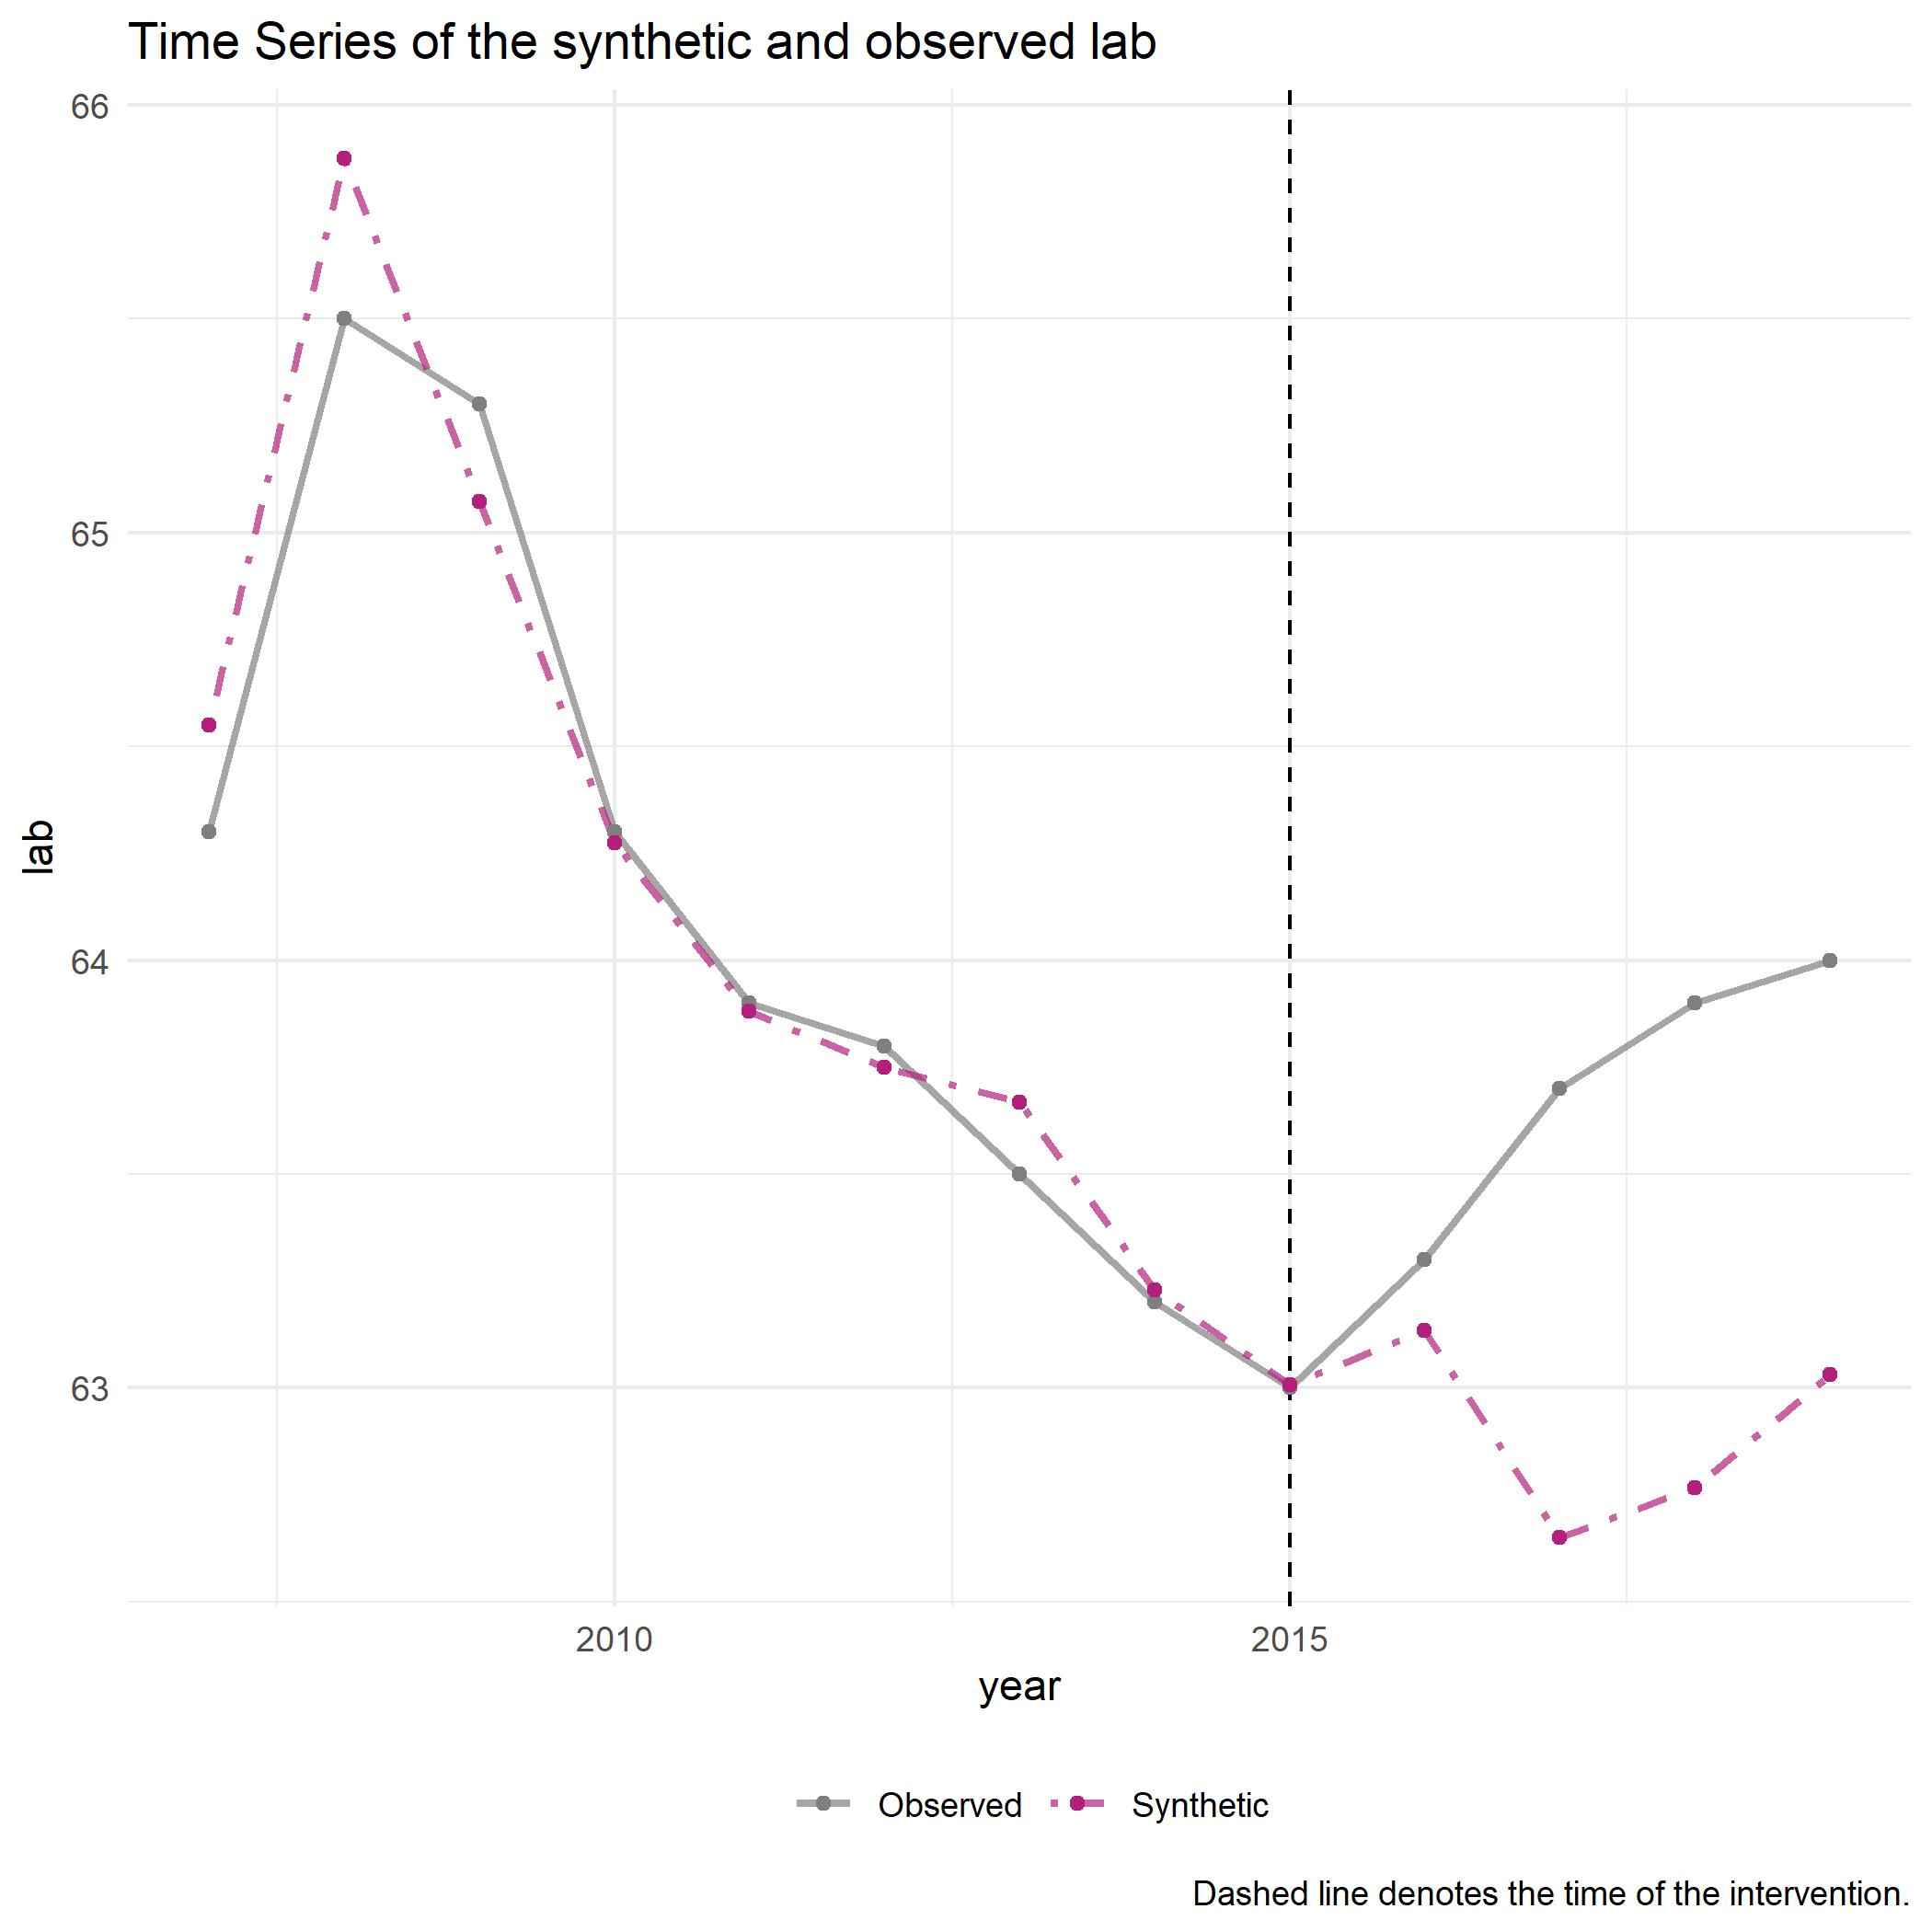
\includegraphics[width=80mm]{ca_lab_trend} &   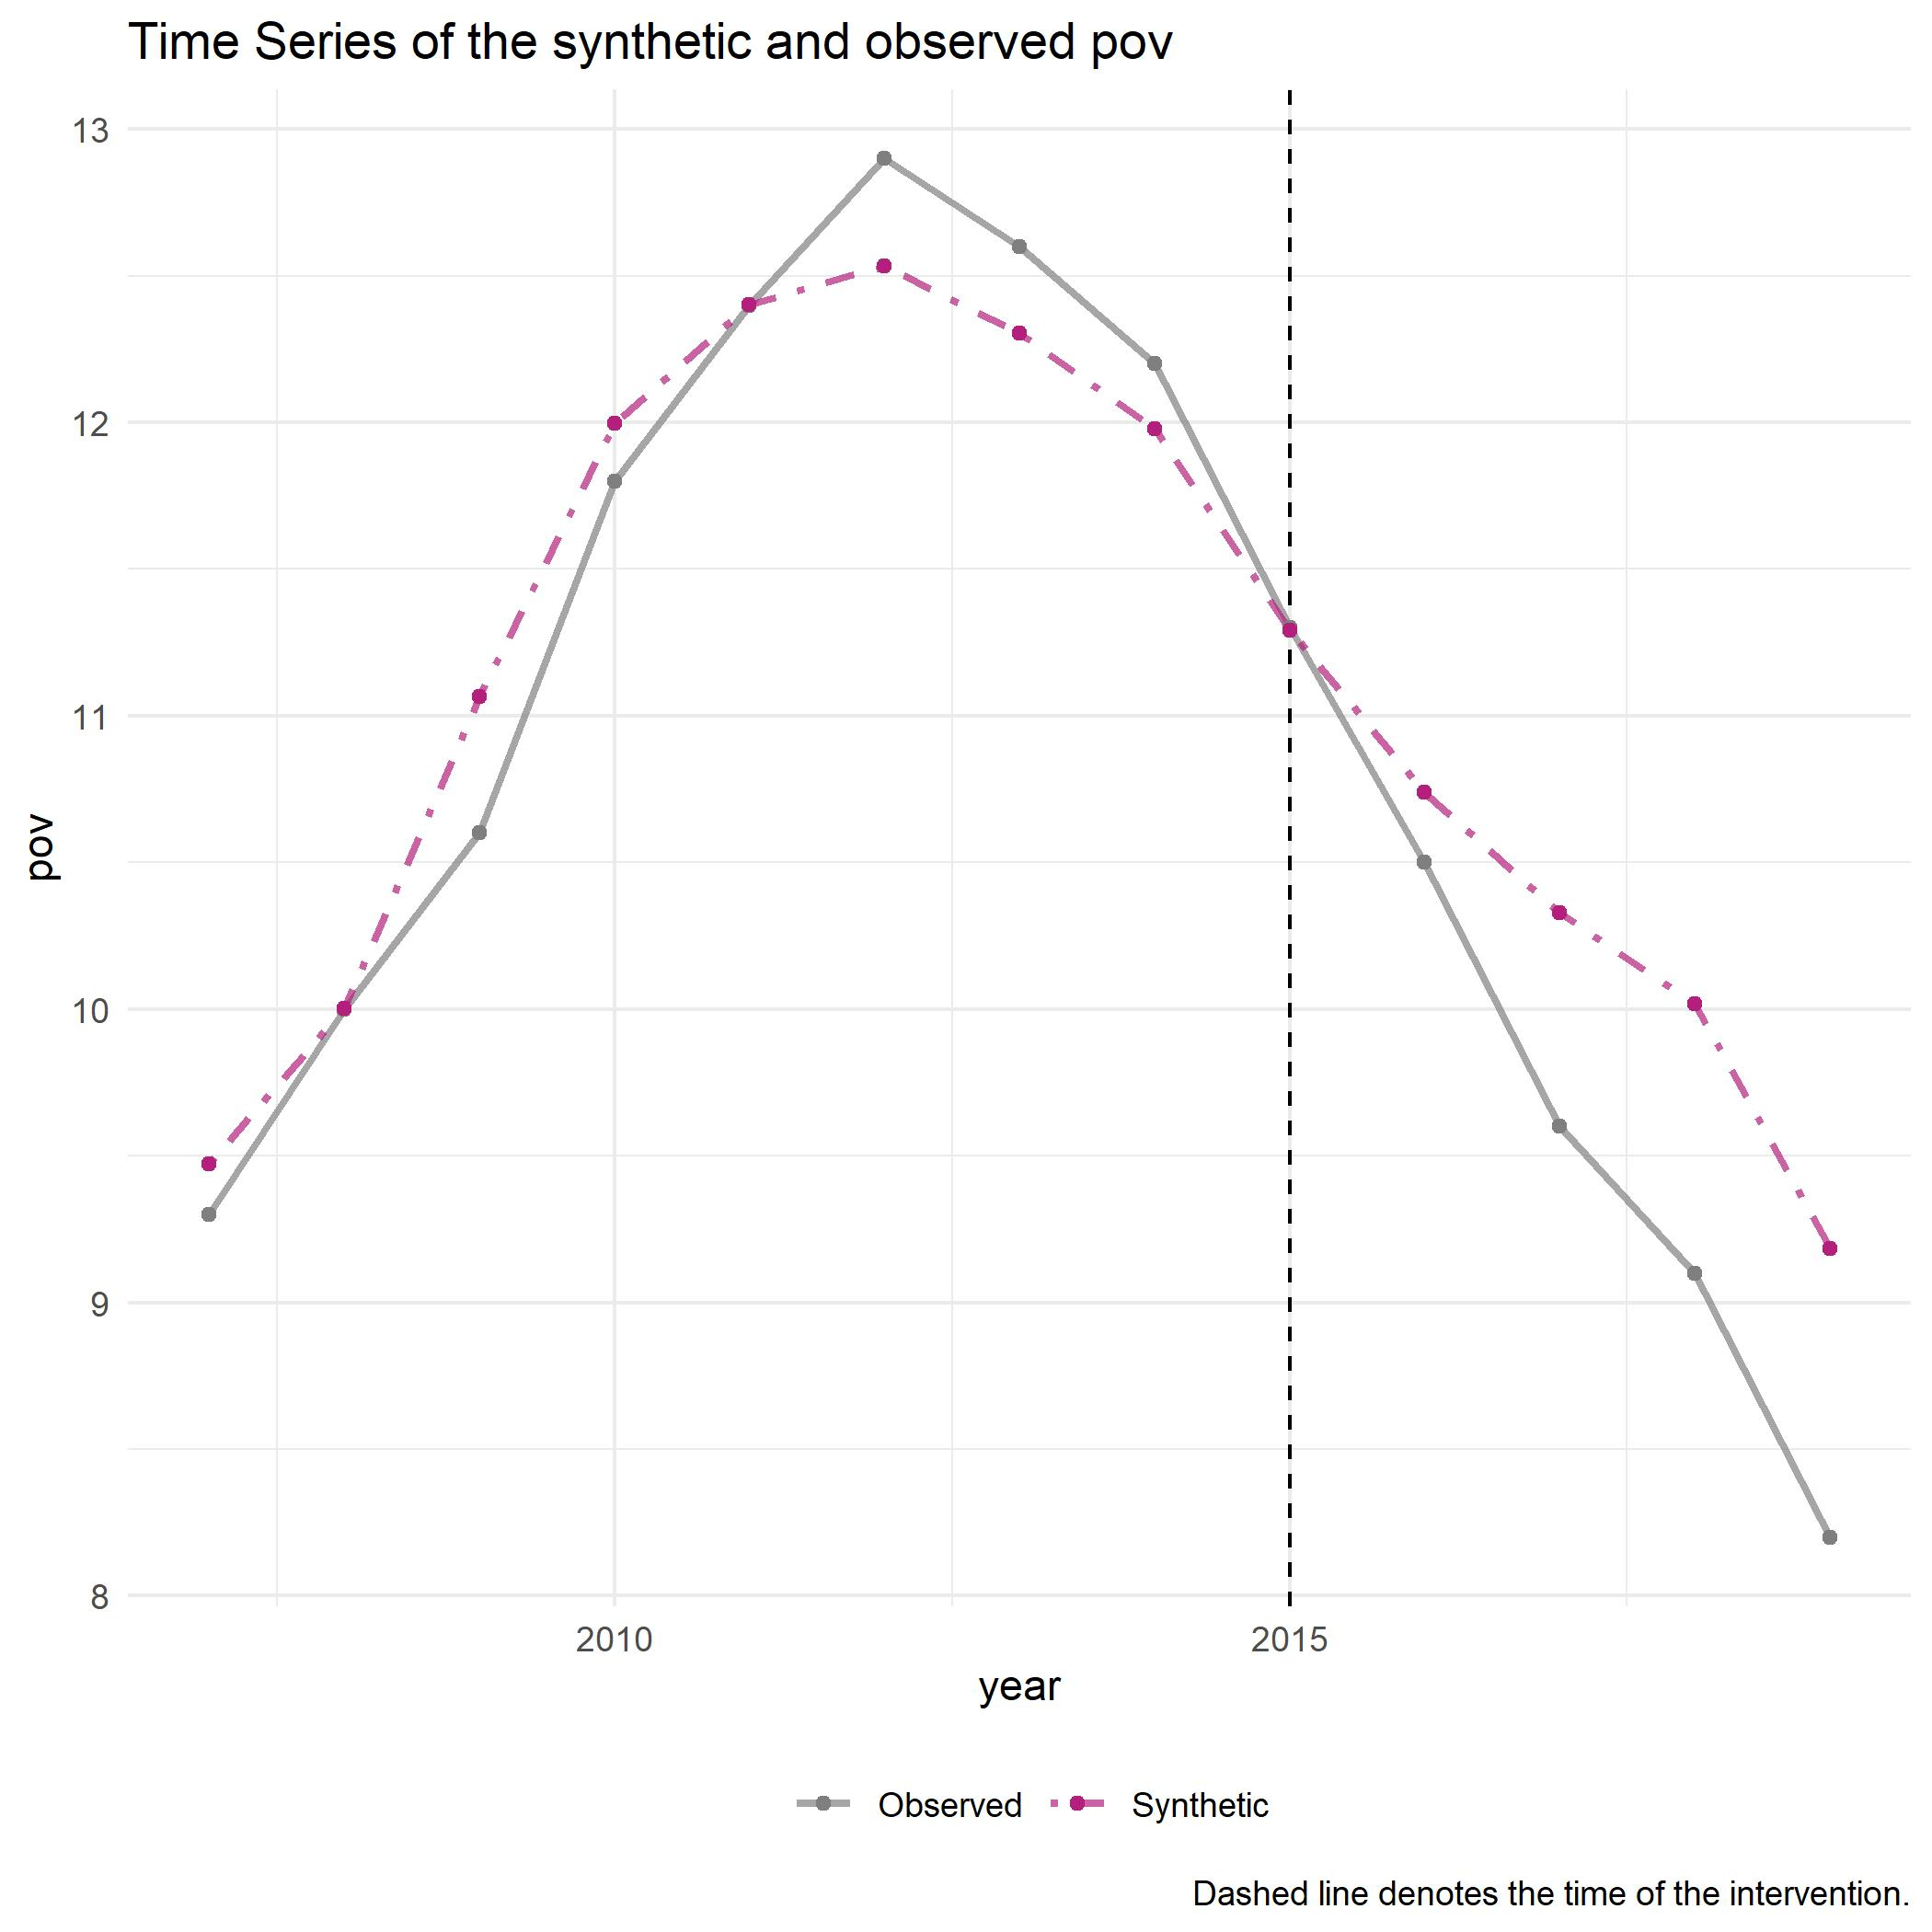
\includegraphics[width=80mm]{ca_pov_trend} \\
 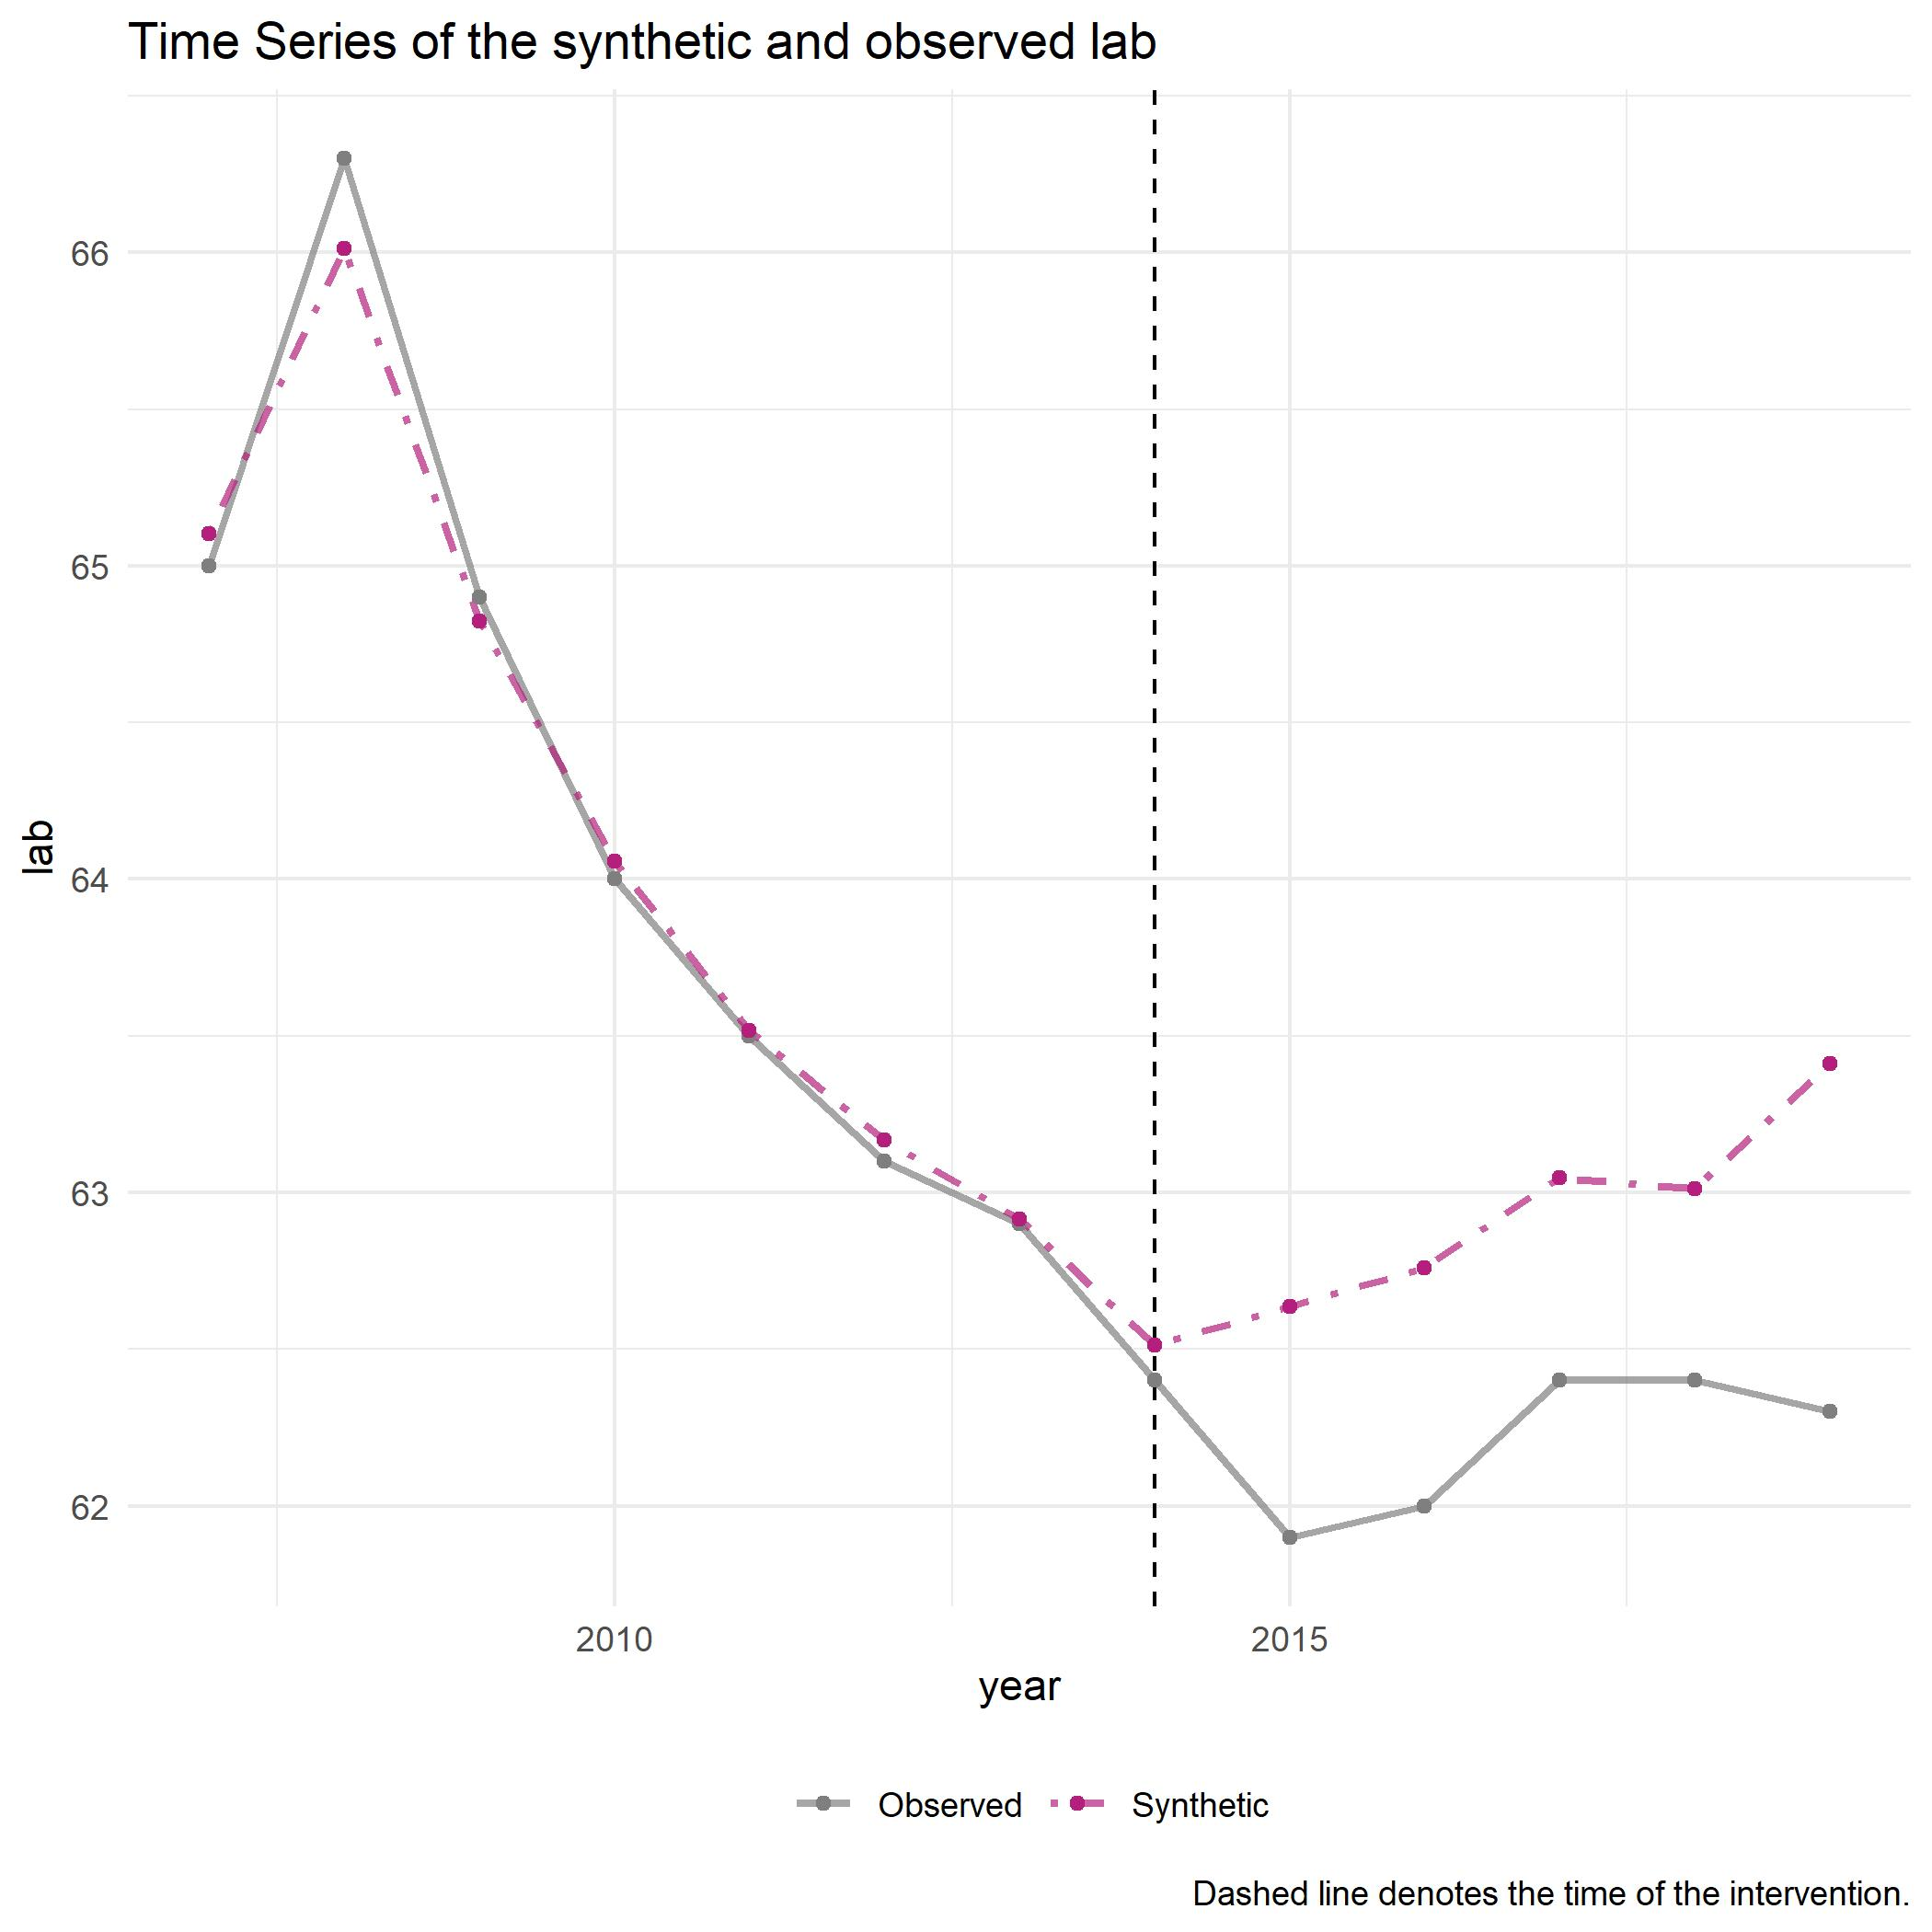
\includegraphics[width=80mm]{nc_lab_trend} &   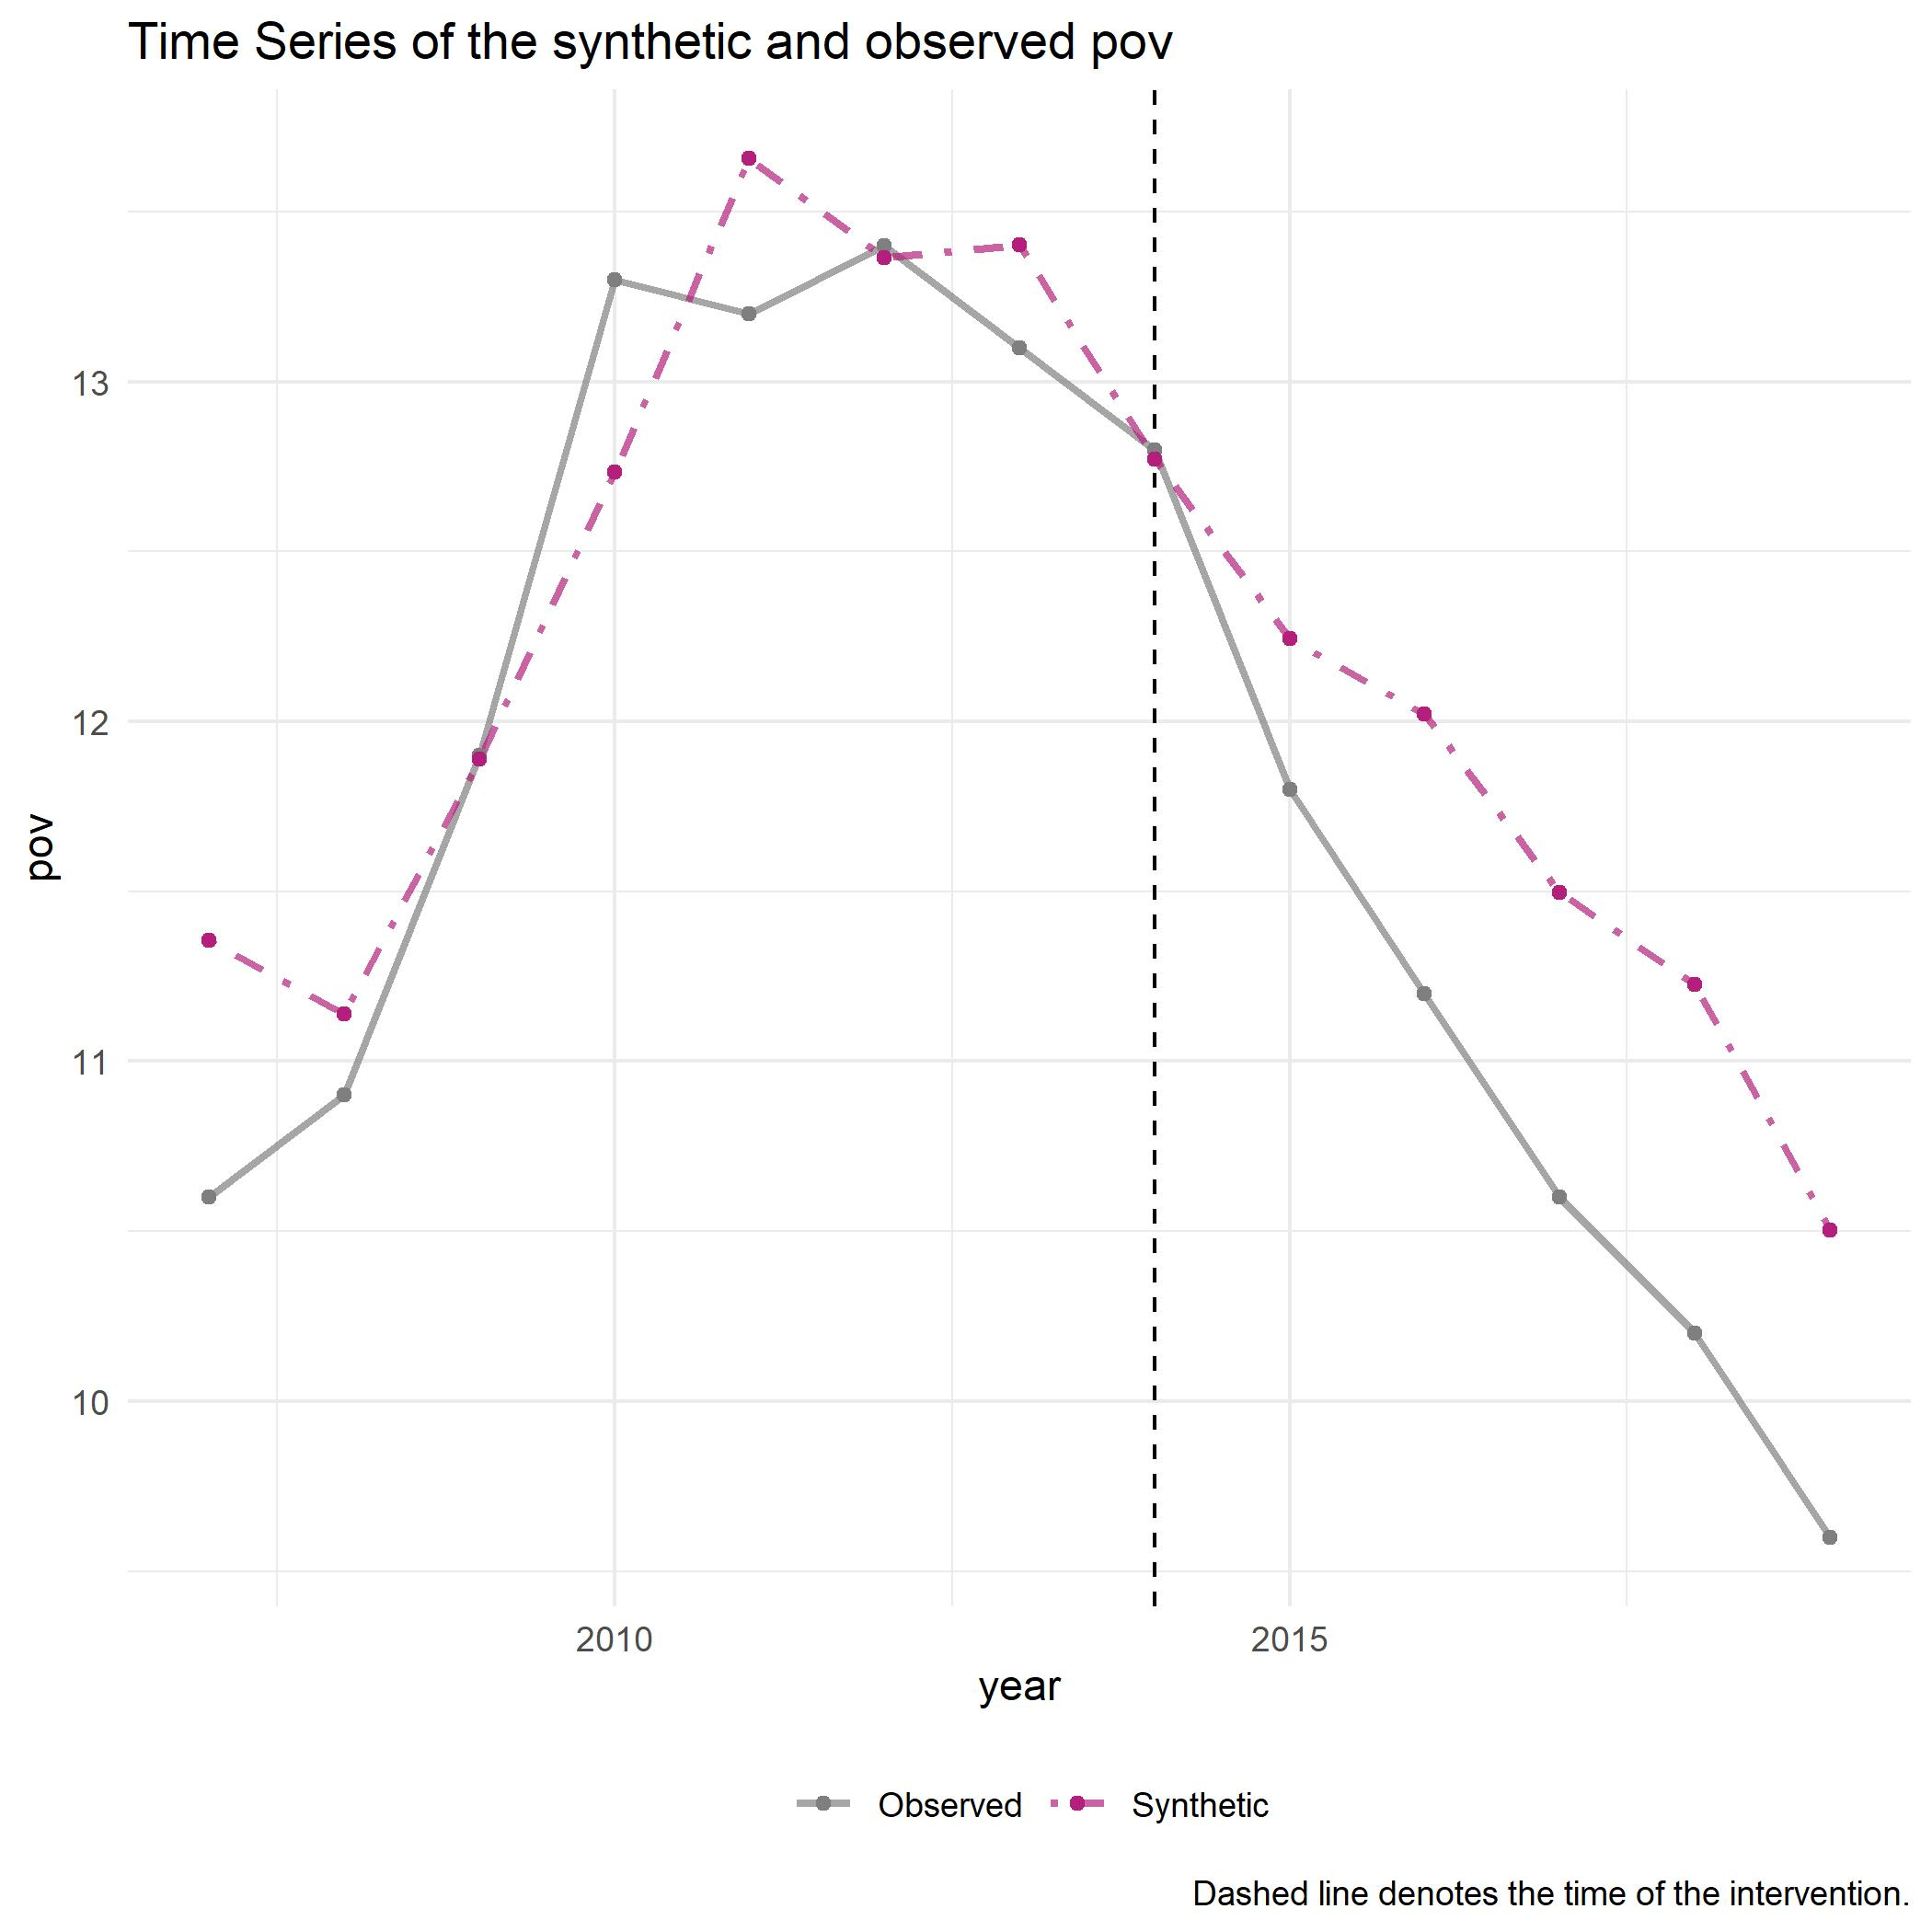
\includegraphics[width=80mm]{nc_pov_trend} \\
\end{tabular}
\end{center}
\end{figure}

\restoregeometry

\newgeometry{margin=.5in}

\begin{figure}
\begin{center}
\caption{Weights Assigned for Synthetic California and North Carolina}
\label{fig:weights}{}
\begin{tabular}{cc}
 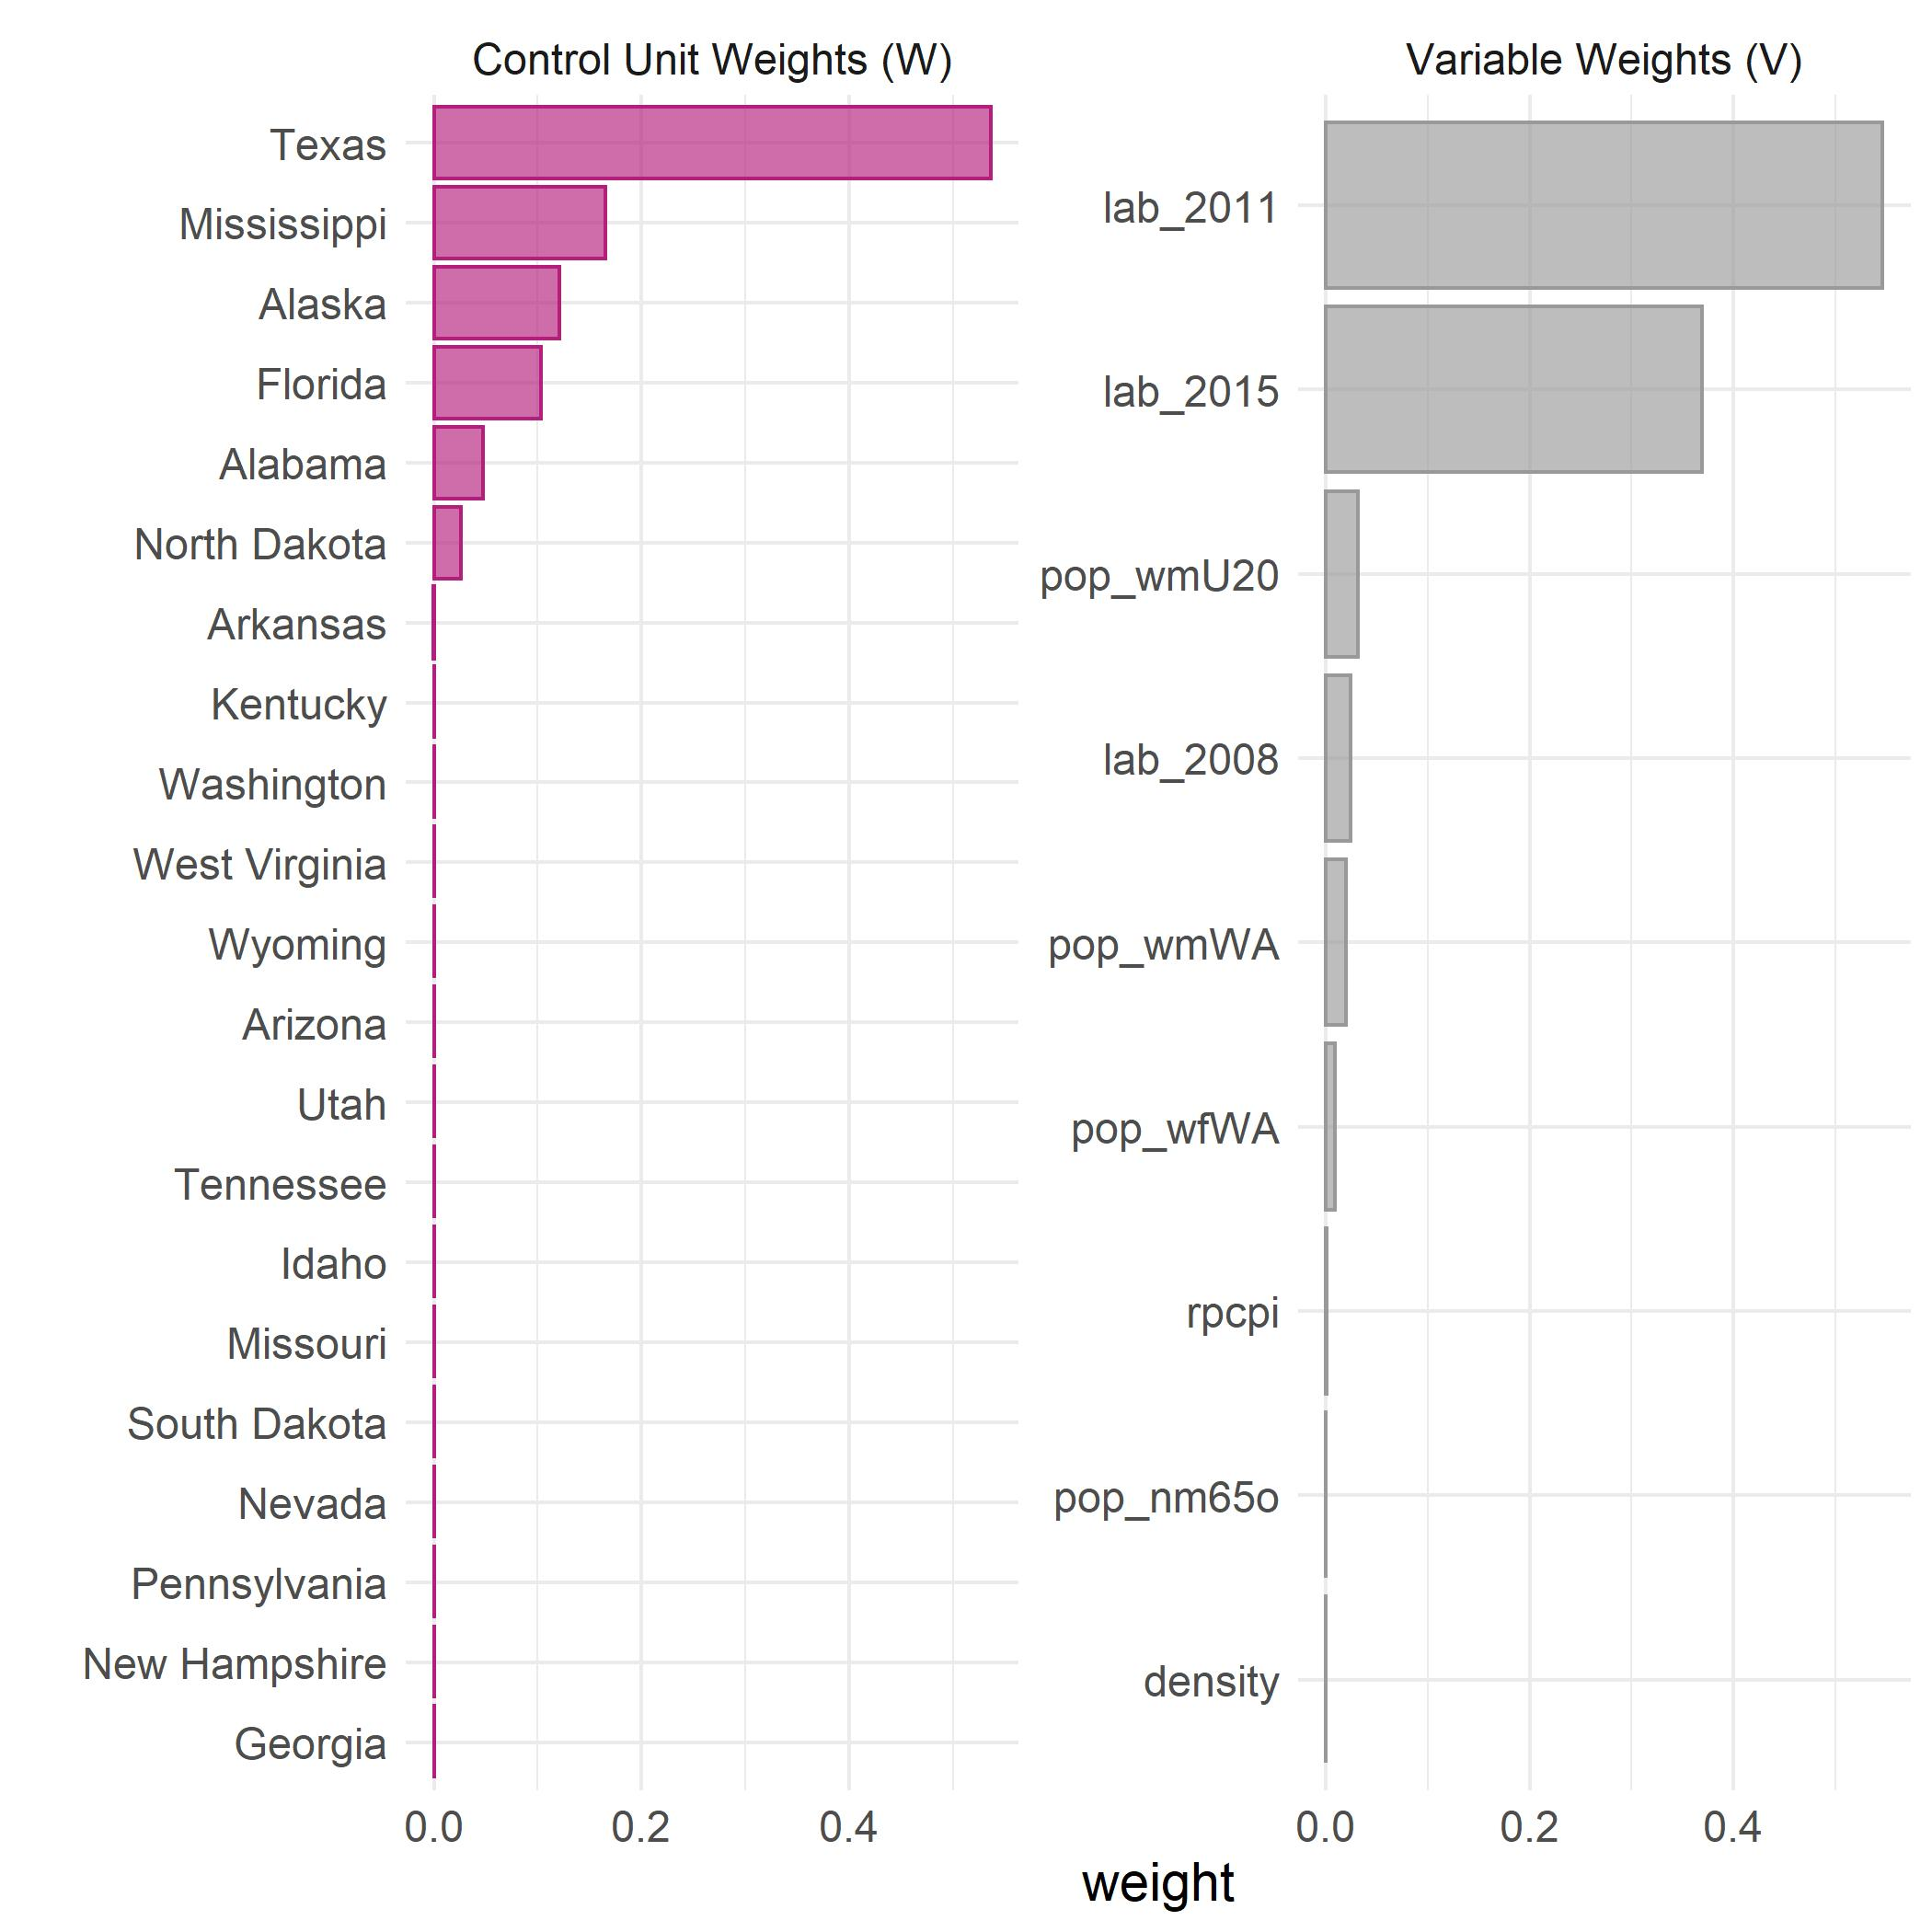
\includegraphics[width=80mm]{ca_lab_weights} &   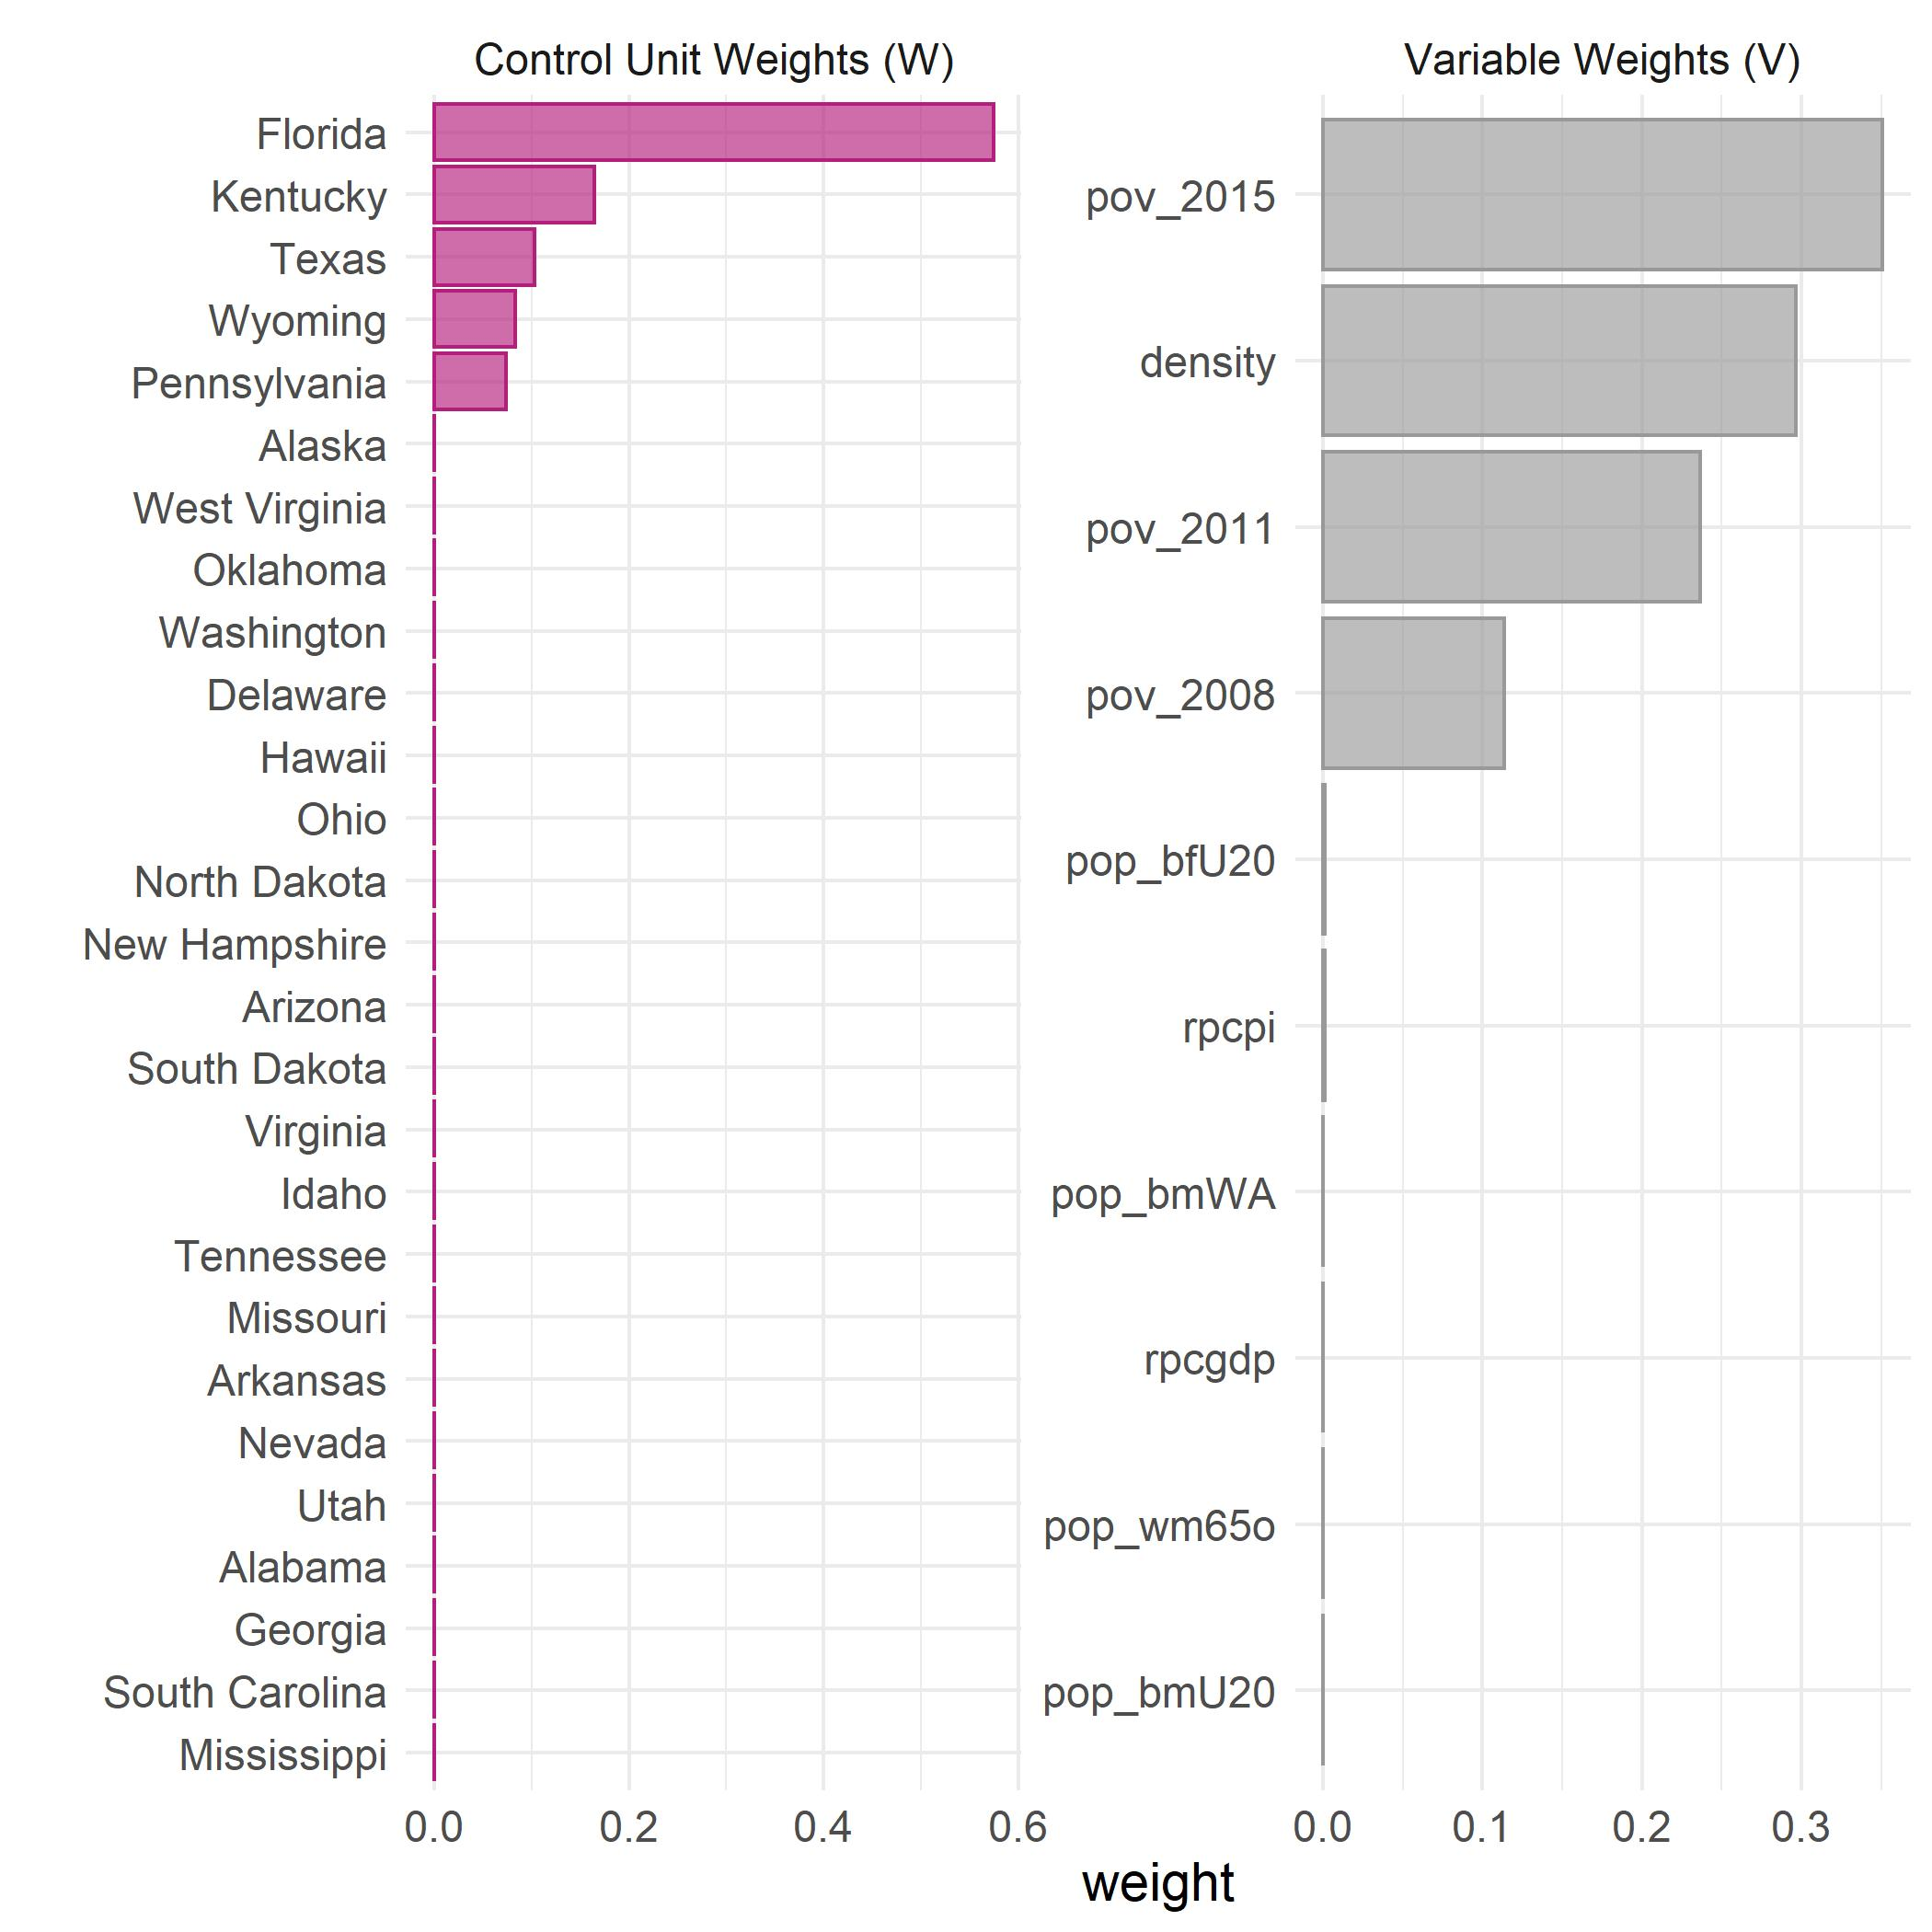
\includegraphics[width=80mm]{ca_pov_weights} \\
 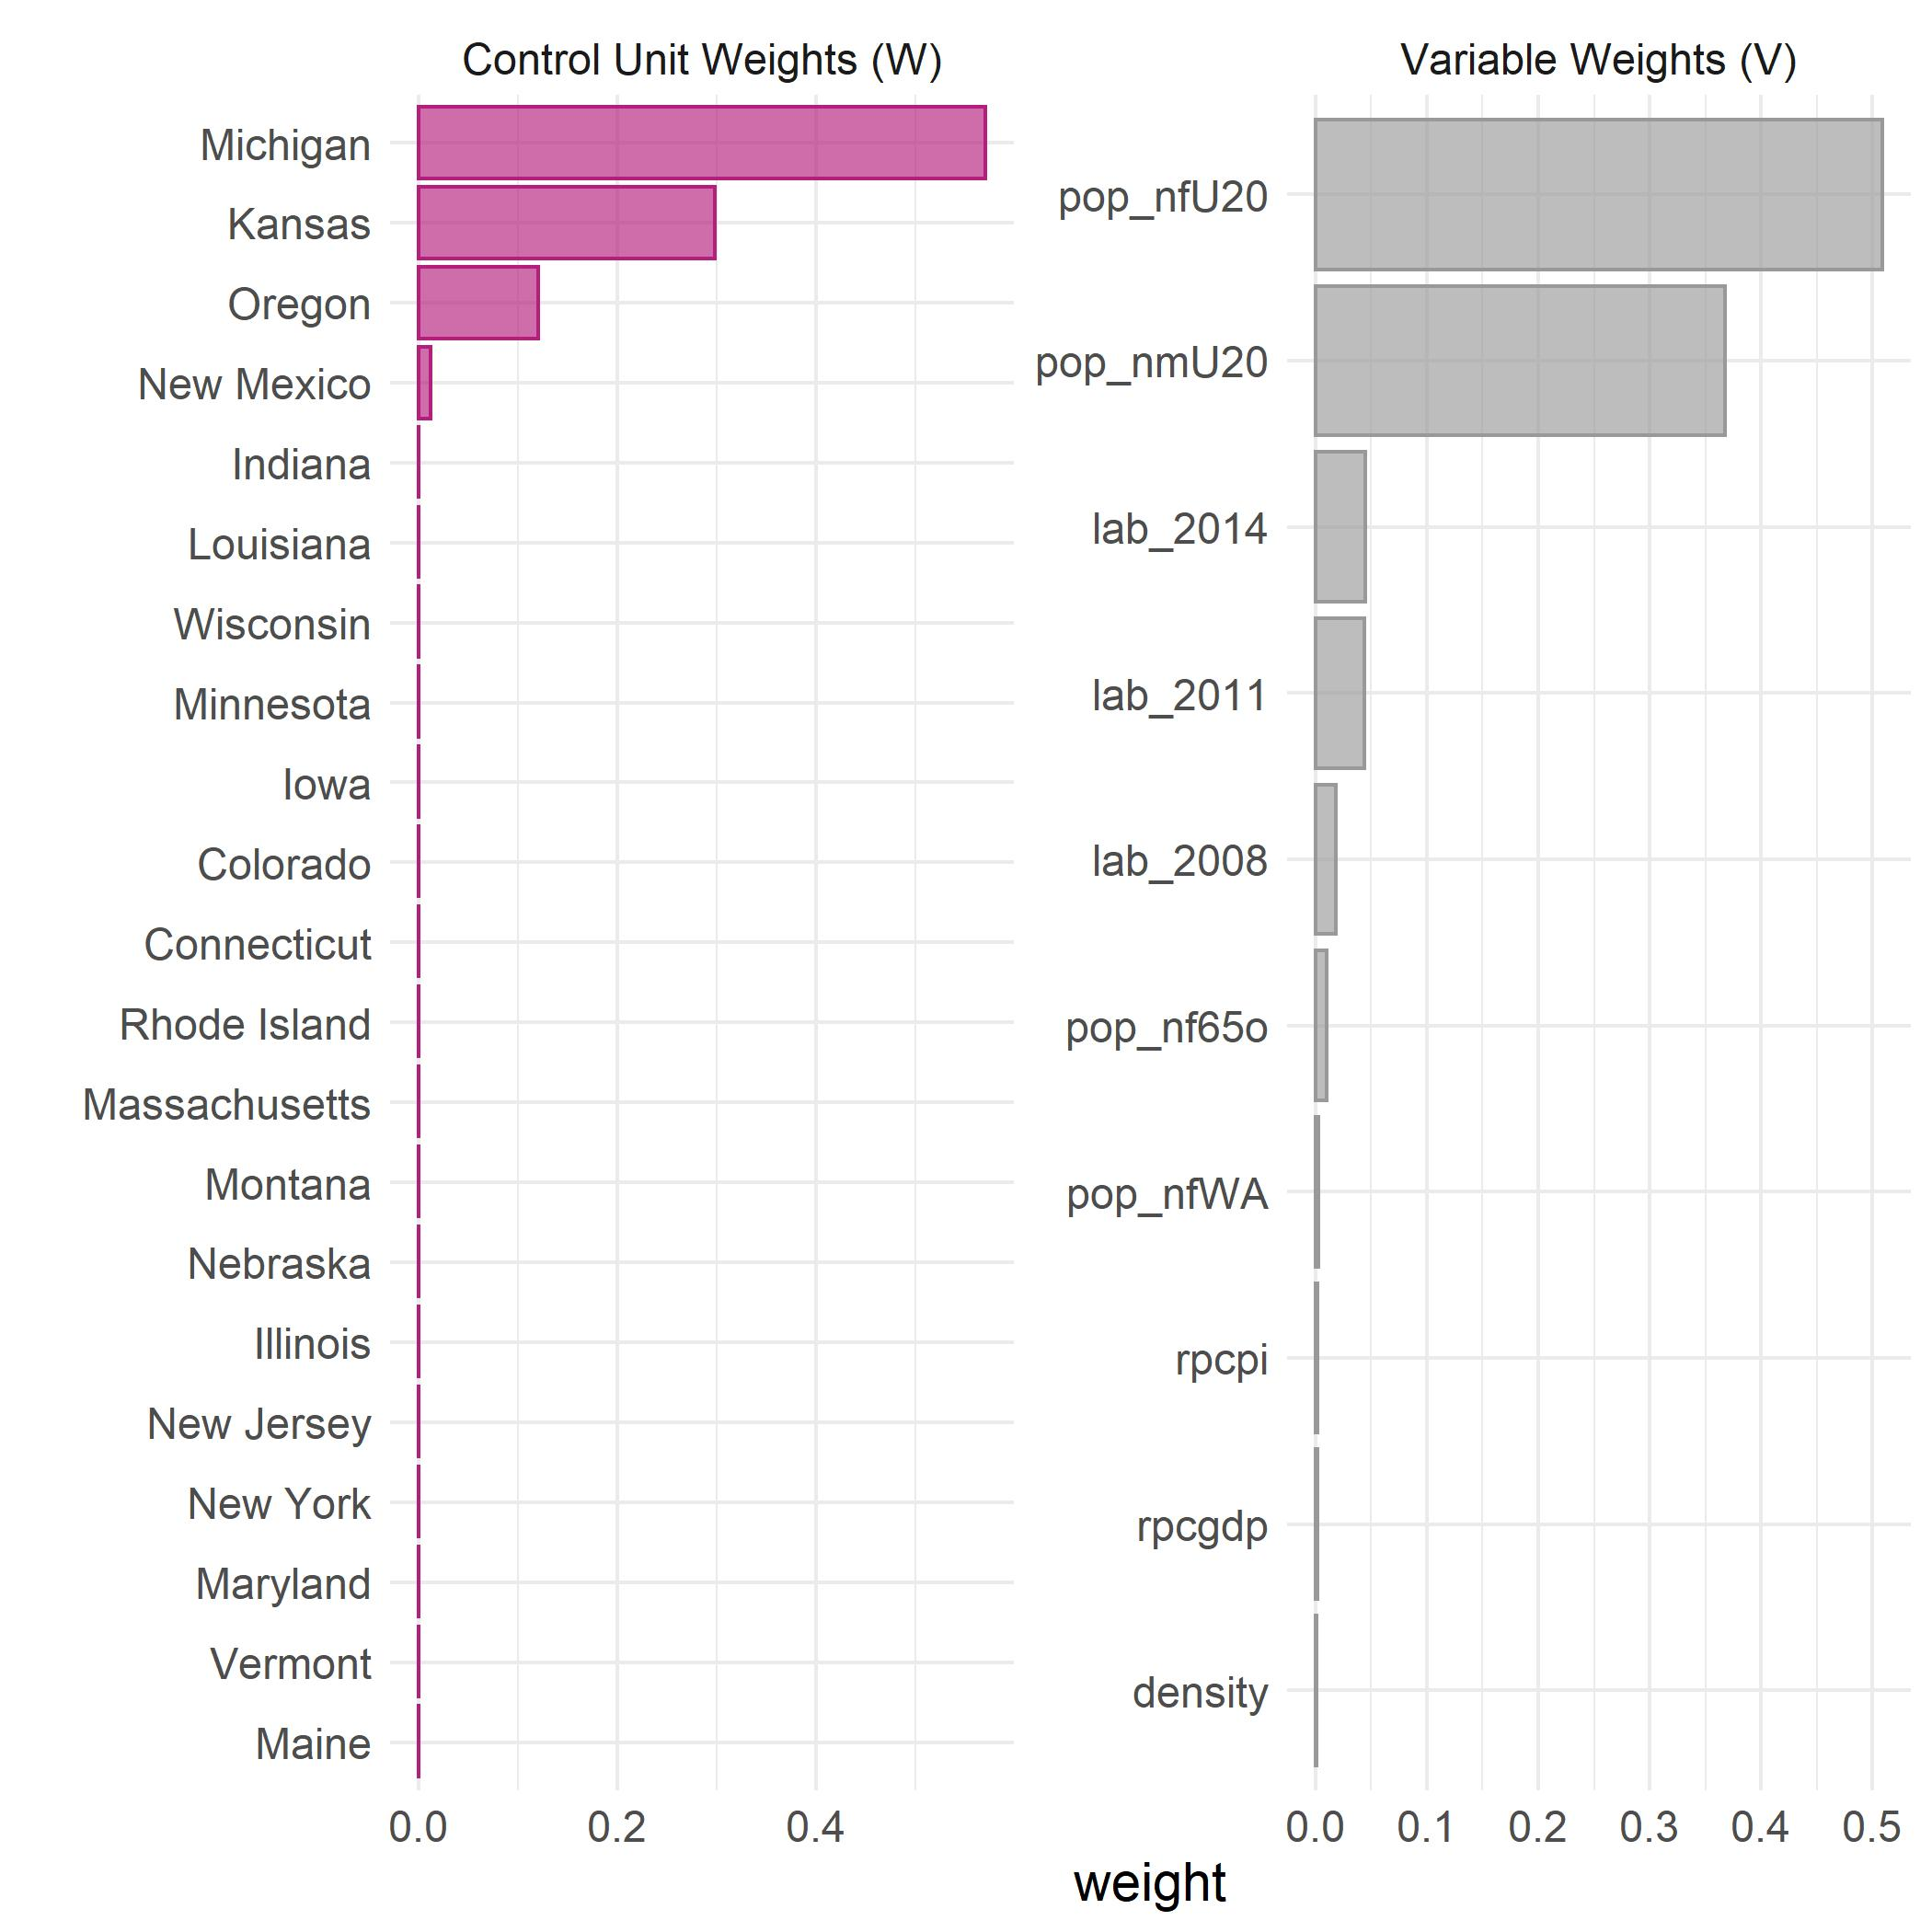
\includegraphics[width=80mm]{nc_lab_weights} &   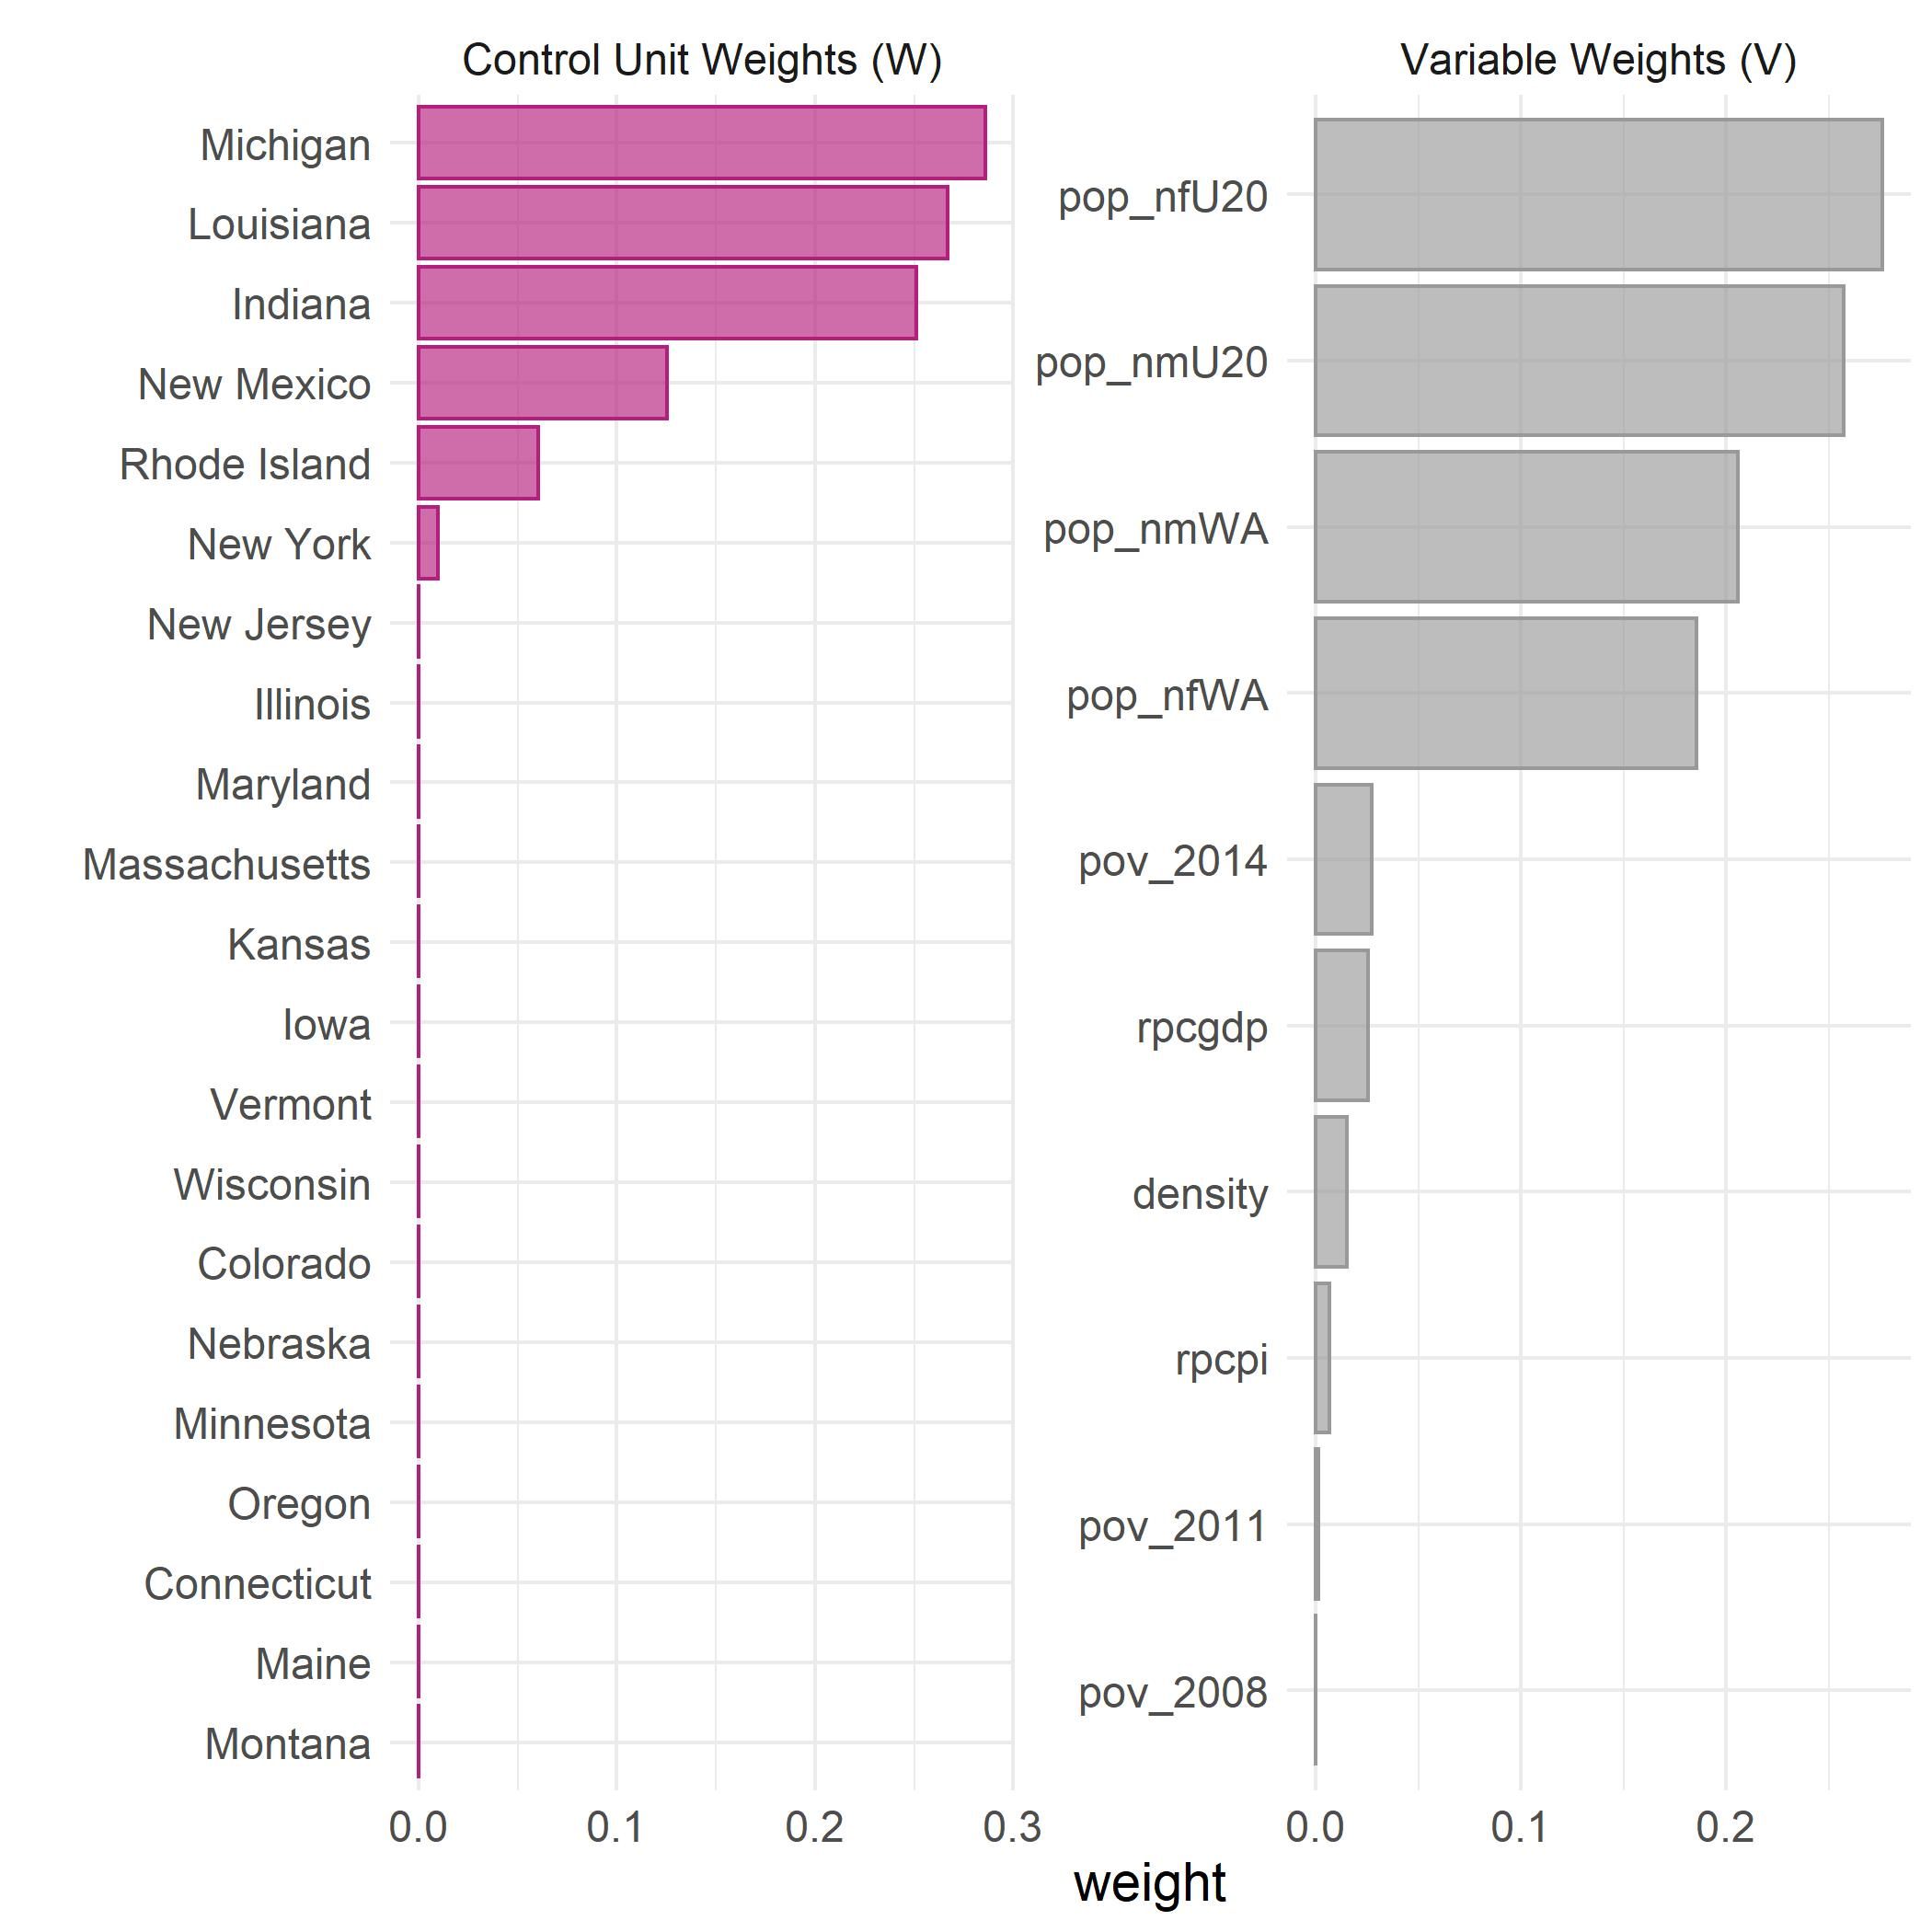
\includegraphics[width=80mm]{nc_pov_weights} \\
\end{tabular}
\end{center}
\end{figure}

\restoregeometry

Figure \ref{fig:diff} allow us to look closely at the difference between the synthetic state and the real state. Following the implementation of CalEITC, we observe a noticeable increase in labor force participation. It peaks at near 1.1\% increase over our synthetic California before returning to a 1\% difference. Conversely, after the elimination of the EITC in North Carolina, there is an observable decrease in labor force participation, deviating below 1\% of synthetic North Carolina. The difference between our observed states and their synthetic counterparts lends some support to the theory that the EITC encourages work at the extensive margin. 

Looking at the effect of our policy on poverty rates, we notice a decrease in poverty rates compared to the control for both California (a 0.8\% decrease), and North Carolina (a 0.75\% decrease). This is puzzling, because while theory would suggest that the adoption of a state-level EITC would reduce poverty as we see in California, North Carolina's results suggest a decrease in poverty after elimination of the EITC. This leads us to a discussion of inference and robustness with synthetic control.  

\restoregeometry

\newgeometry{margin=.5in}

\begin{figure}
\begin{center}
\caption{Difference Between Synthetic State and Real State}
\label{fig:diff}{}
\begin{tabular}{cc}
 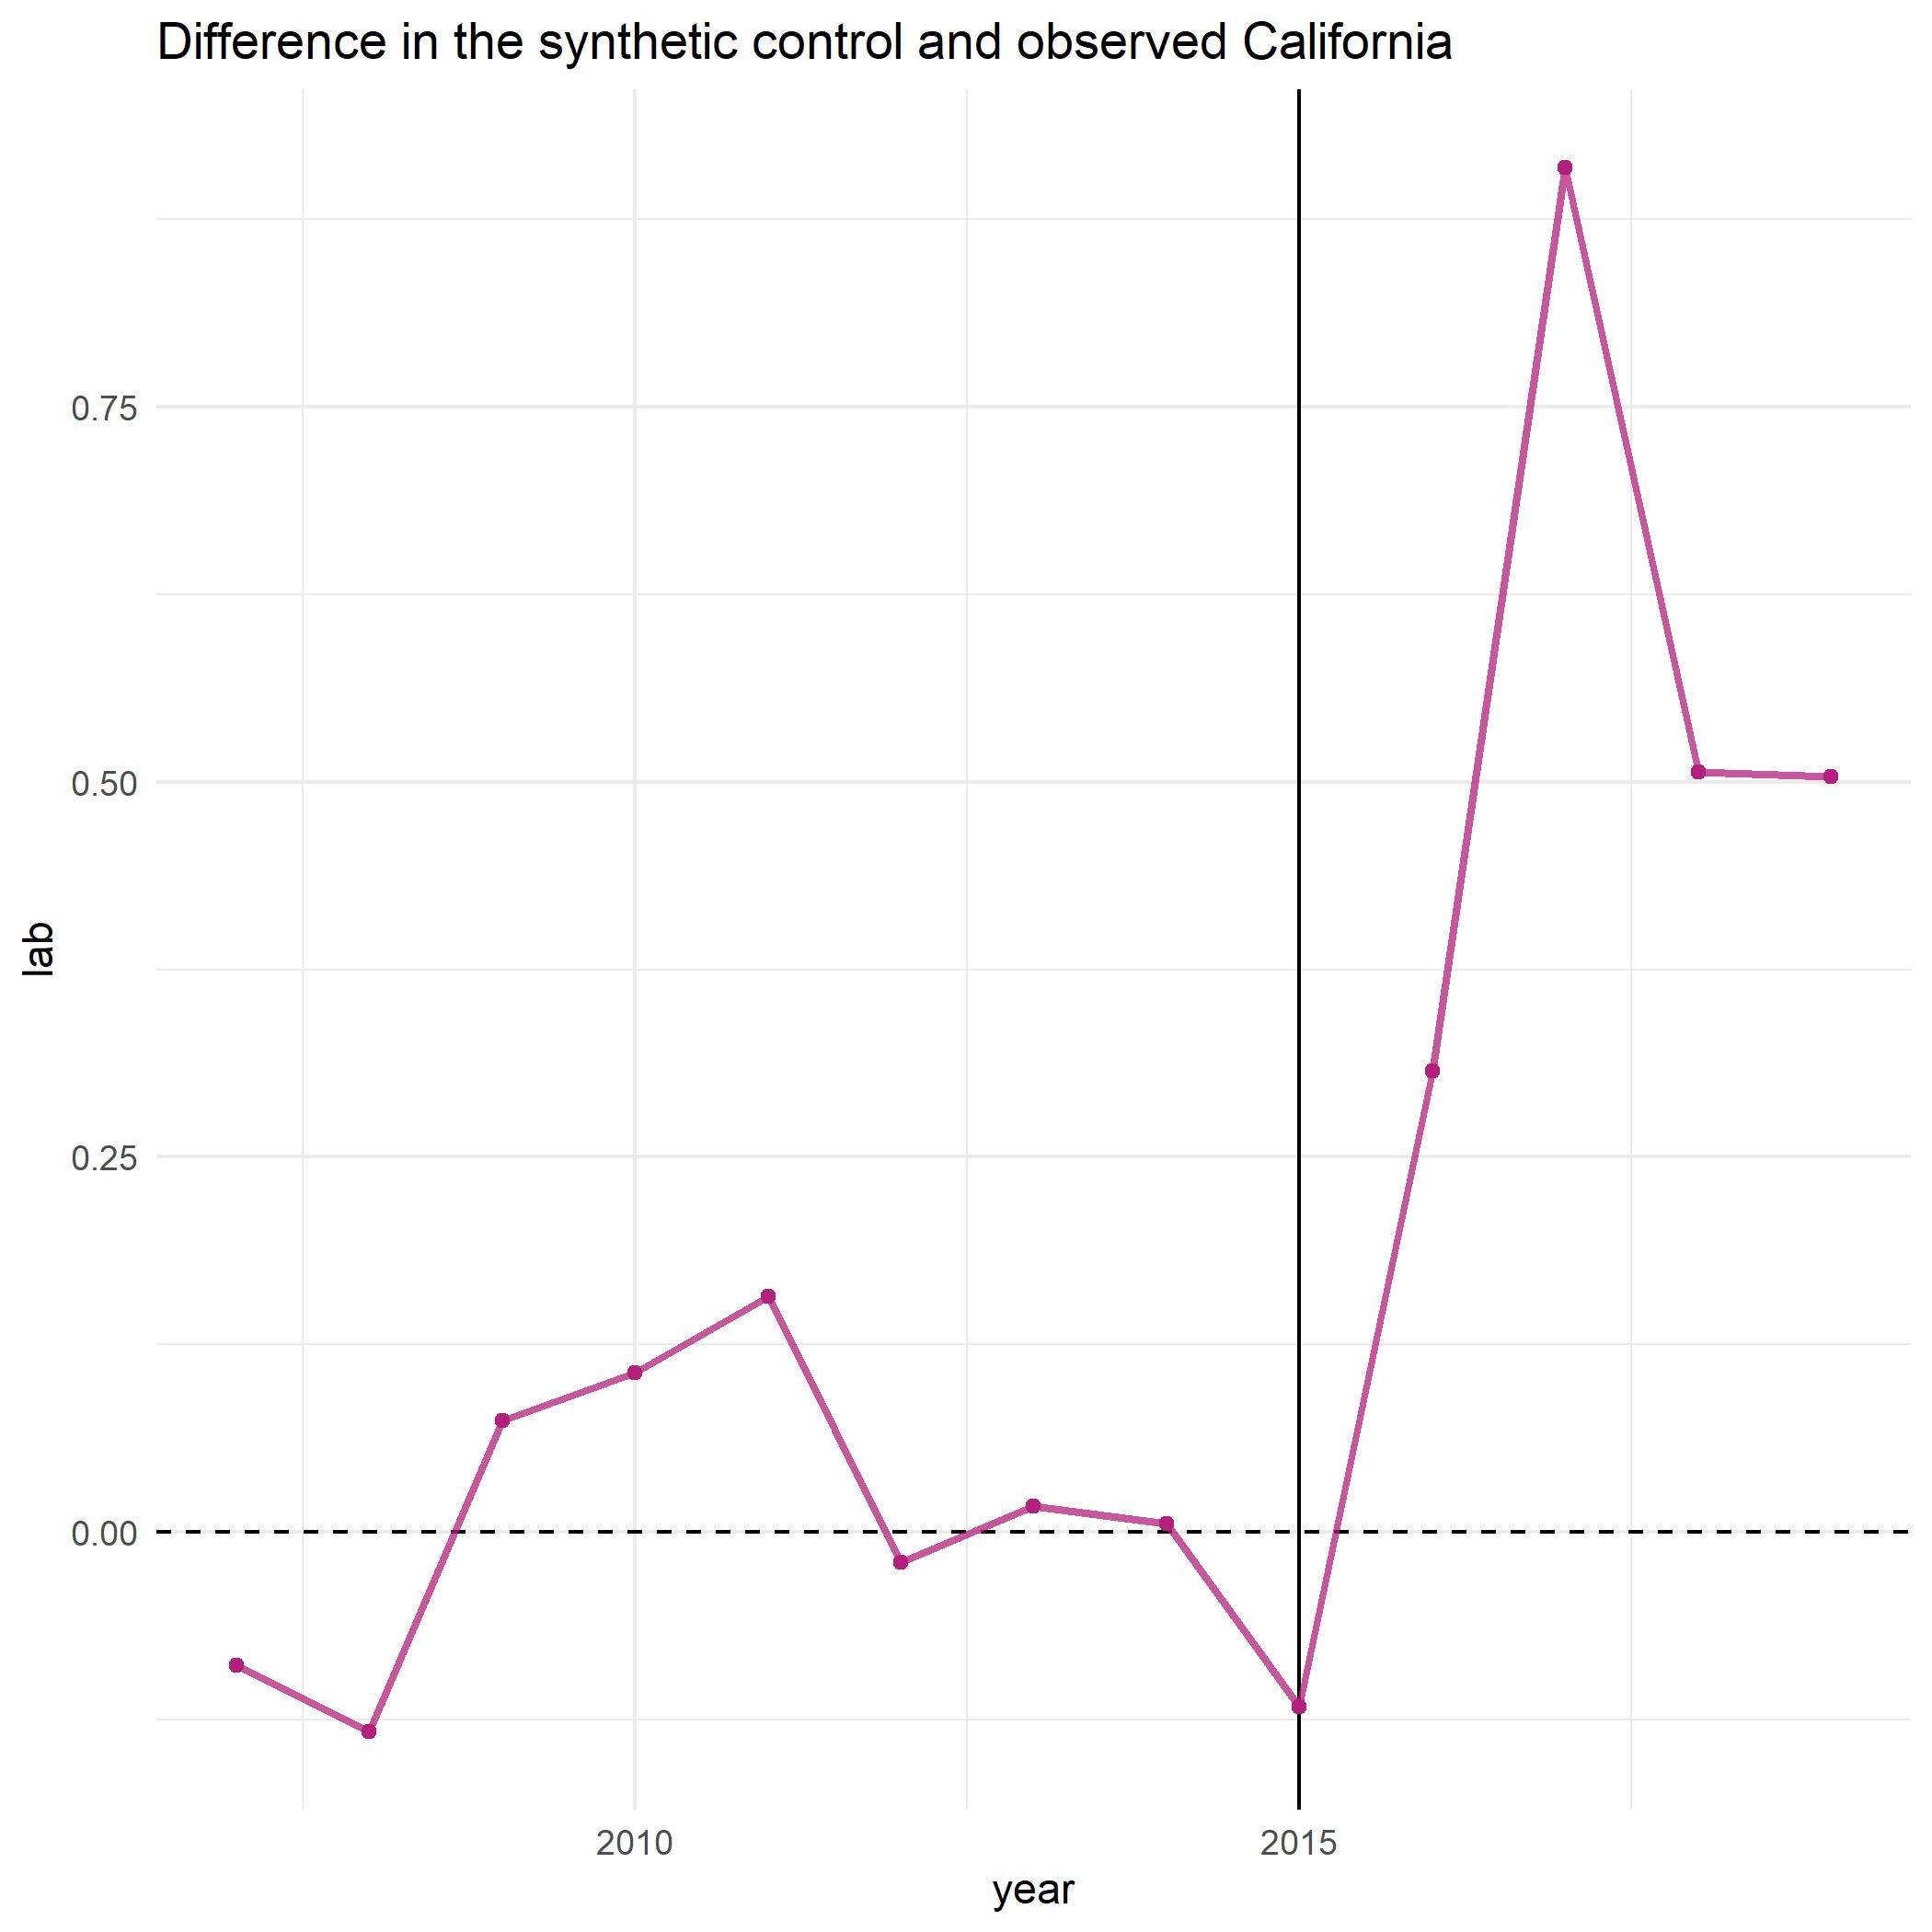
\includegraphics[width=80mm]{ca_lab_diff} &   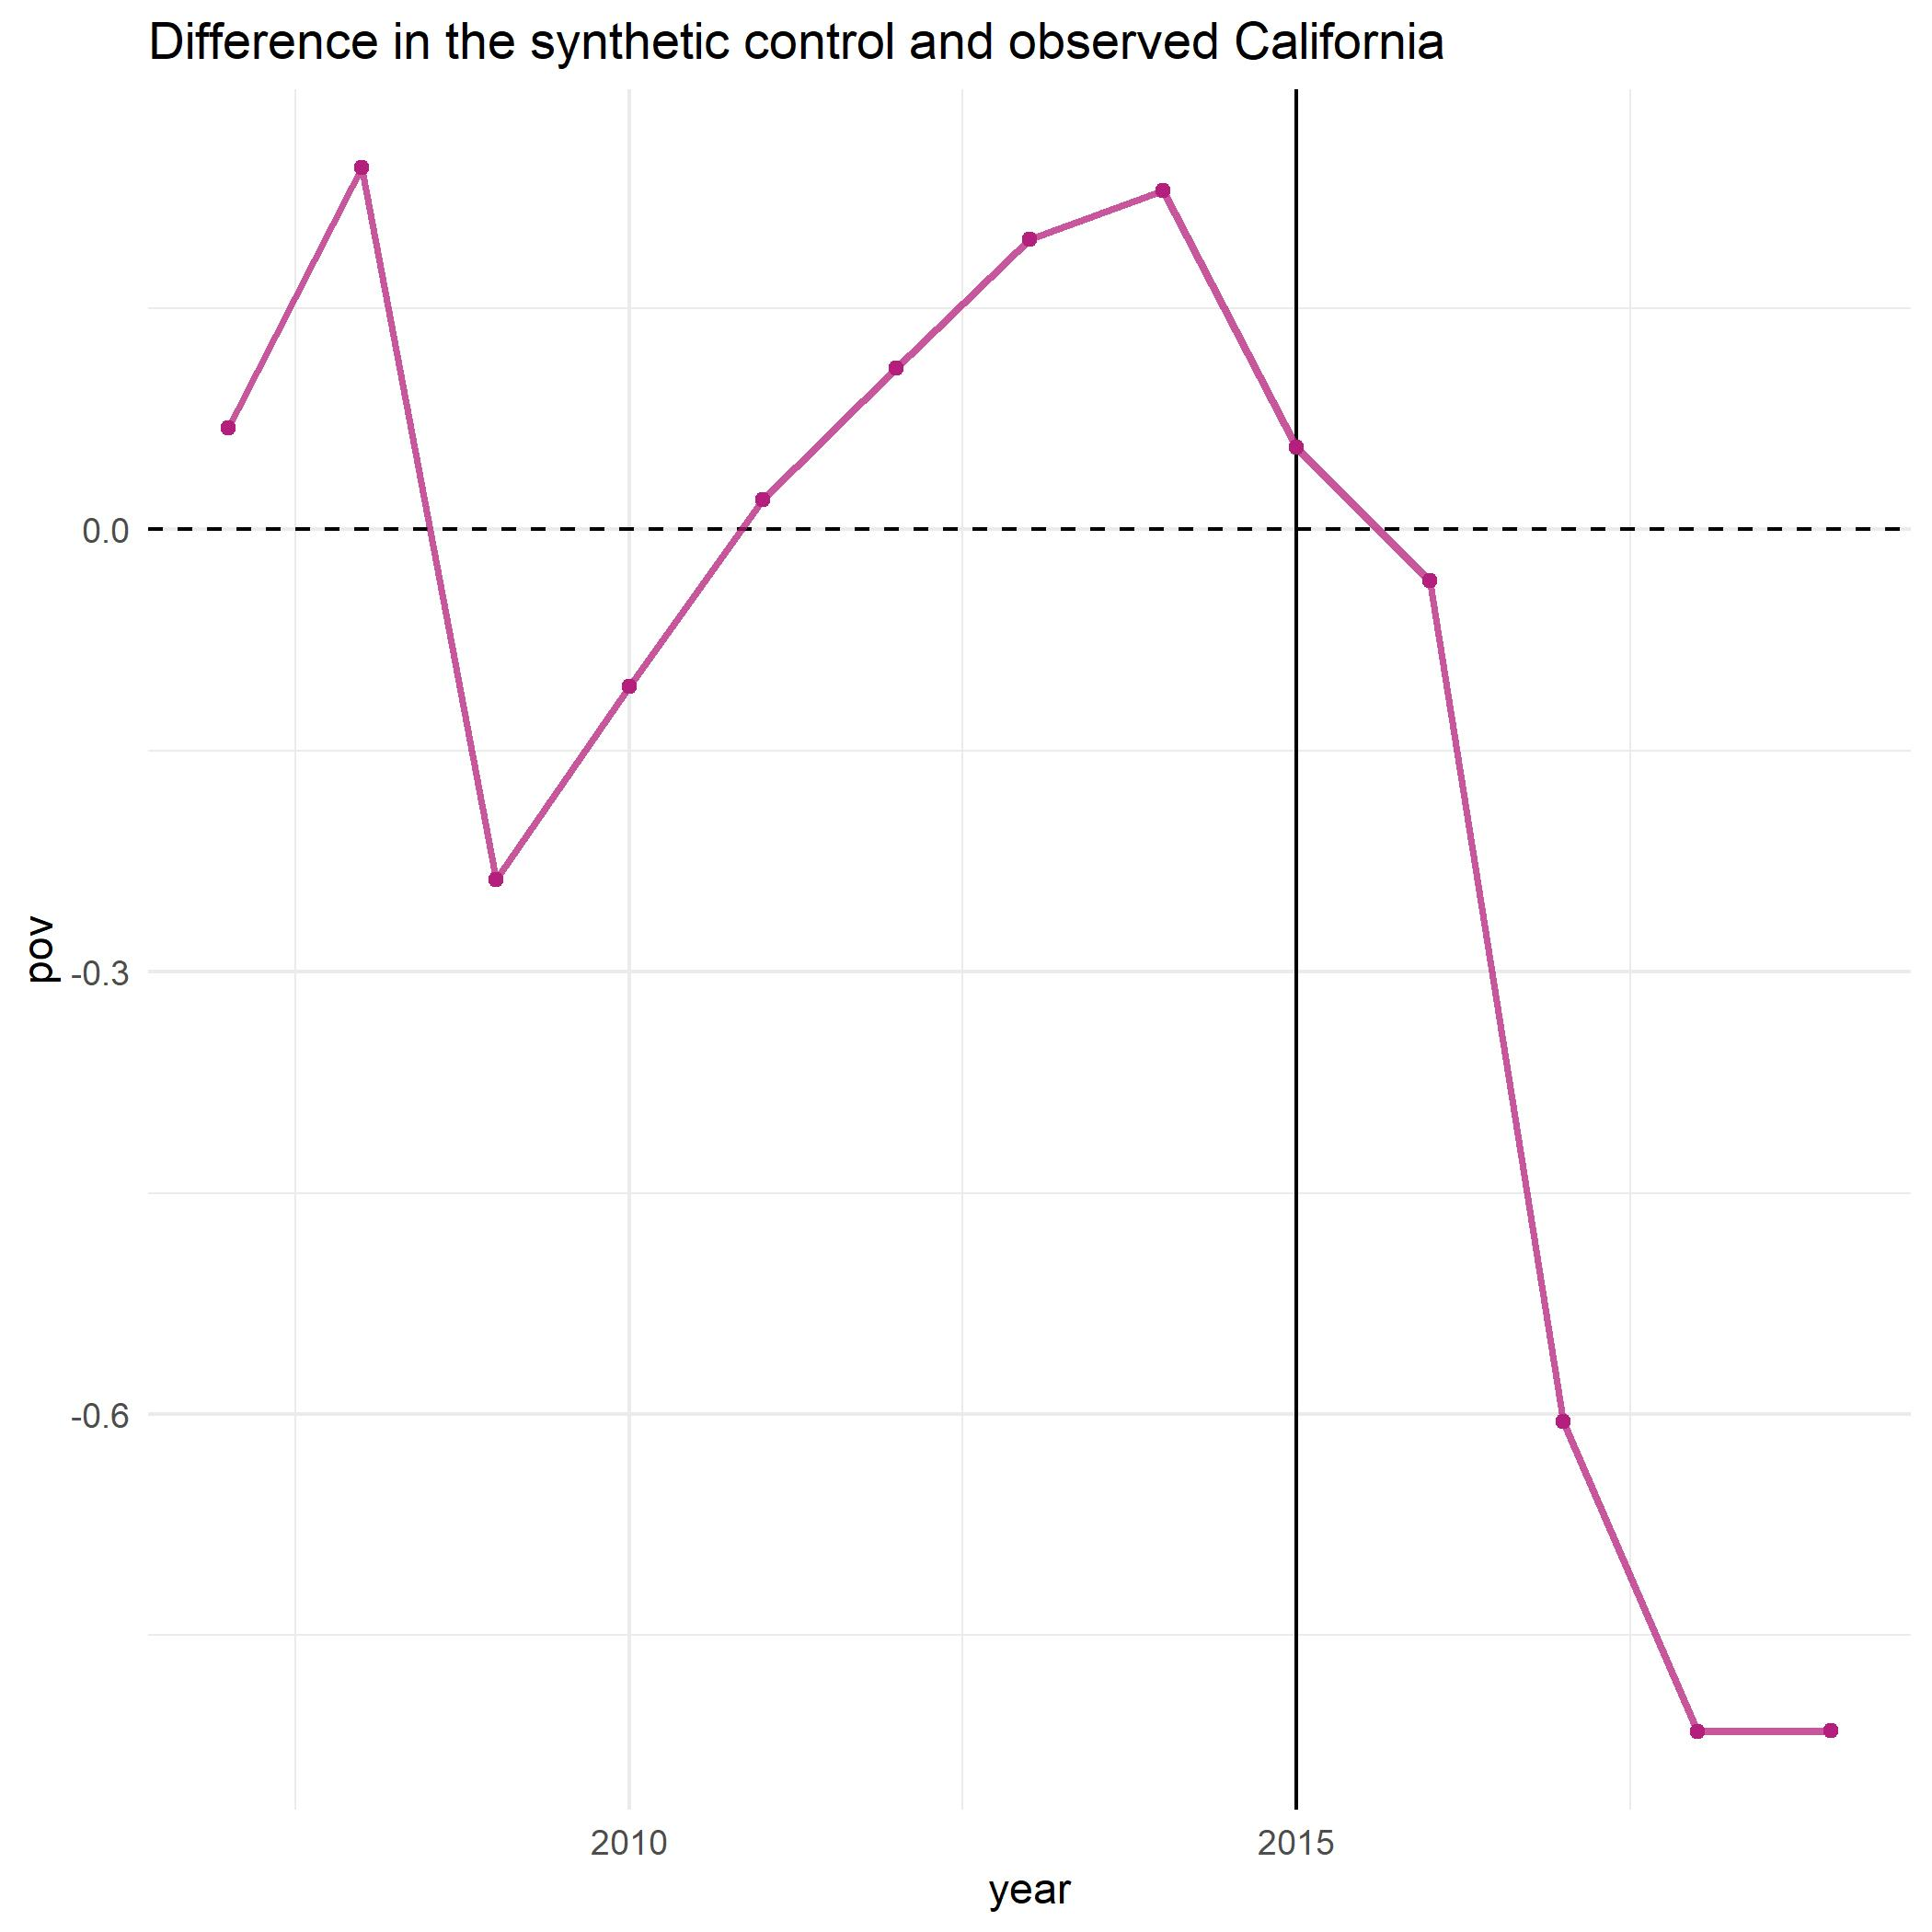
\includegraphics[width=80mm]{ca_pov_diff} \\
 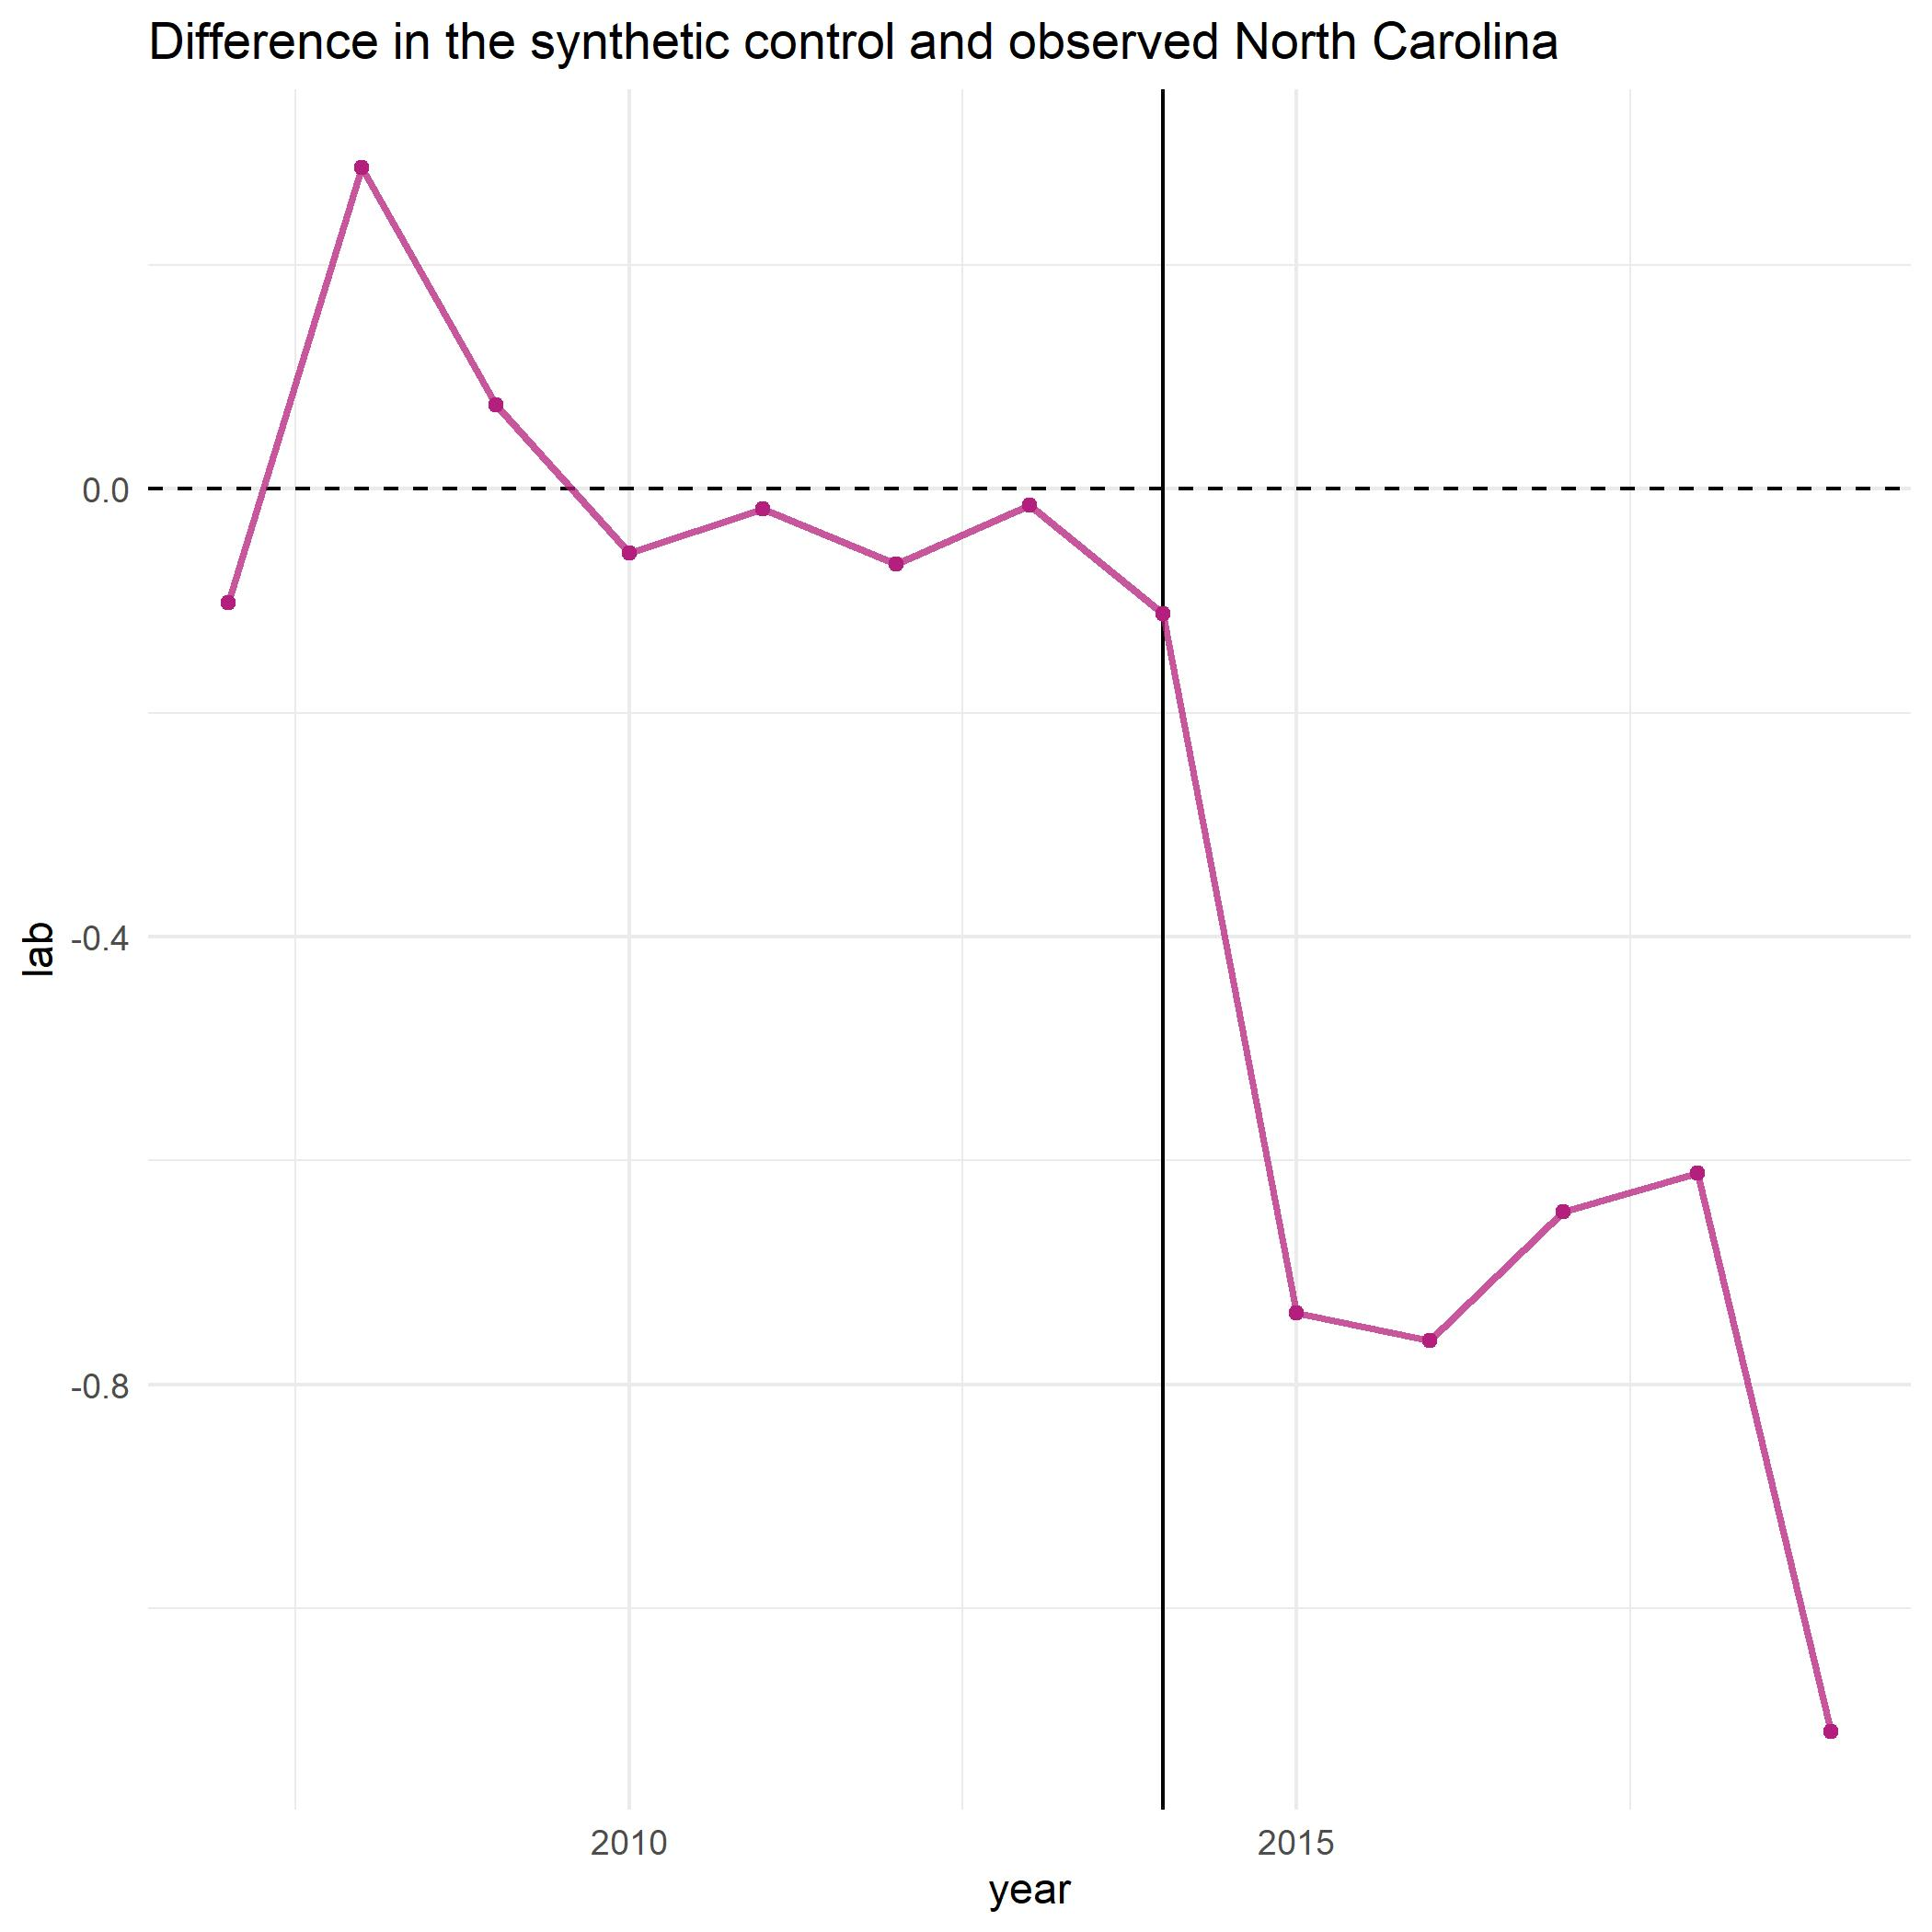
\includegraphics[width=80mm]{nc_lab_diff} &   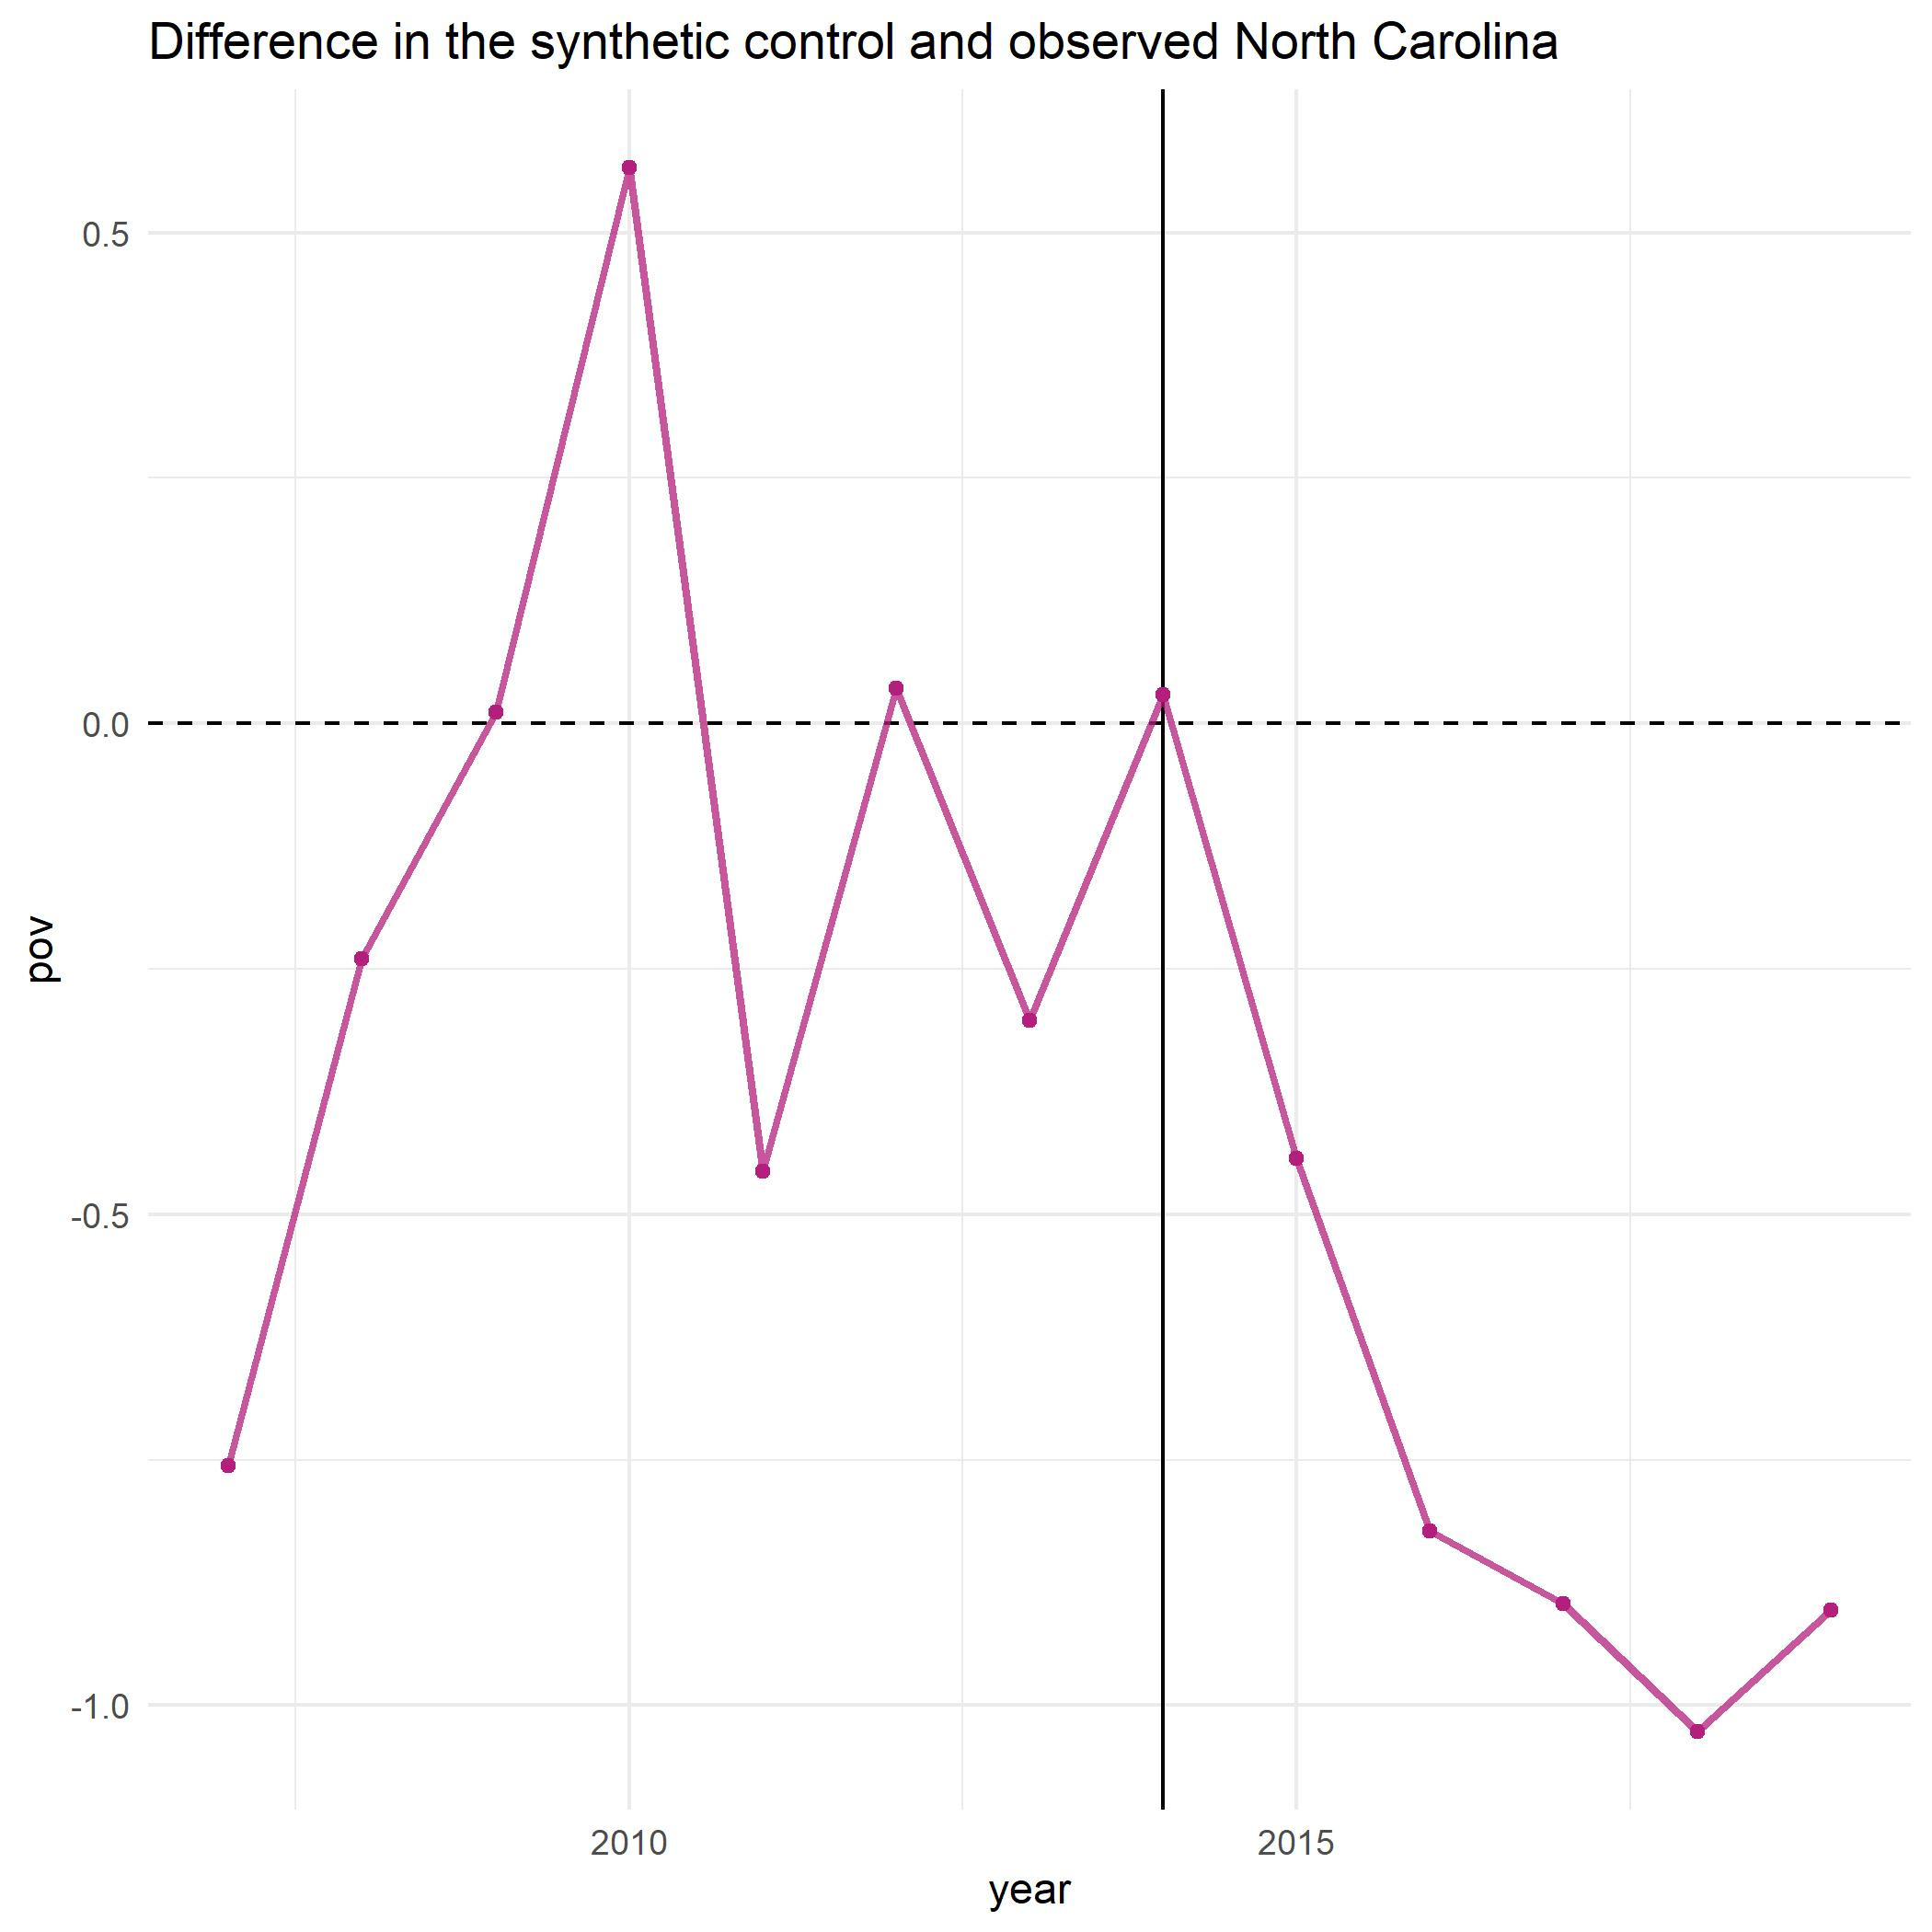
\includegraphics[width=80mm]{nc_pov_diff} \\
\end{tabular}
\end{center}
\end{figure}

\restoregeometry

In order to test the significance of these results, we generate a series of placebos by repeating our synthetic control model on each state in the control group, and compare the results of the placebos to the results we have seen in figures \ref{fig:series} and \ref{fig:diff}. This allows us to determine if we are indeed detecting a causal effect of a policy, or if our results could be generated by chance. 


 \begin{figure}[H]
    \caption{Poverty Gap in California and Poverty Placebo Gaps}
    \begin{center}
        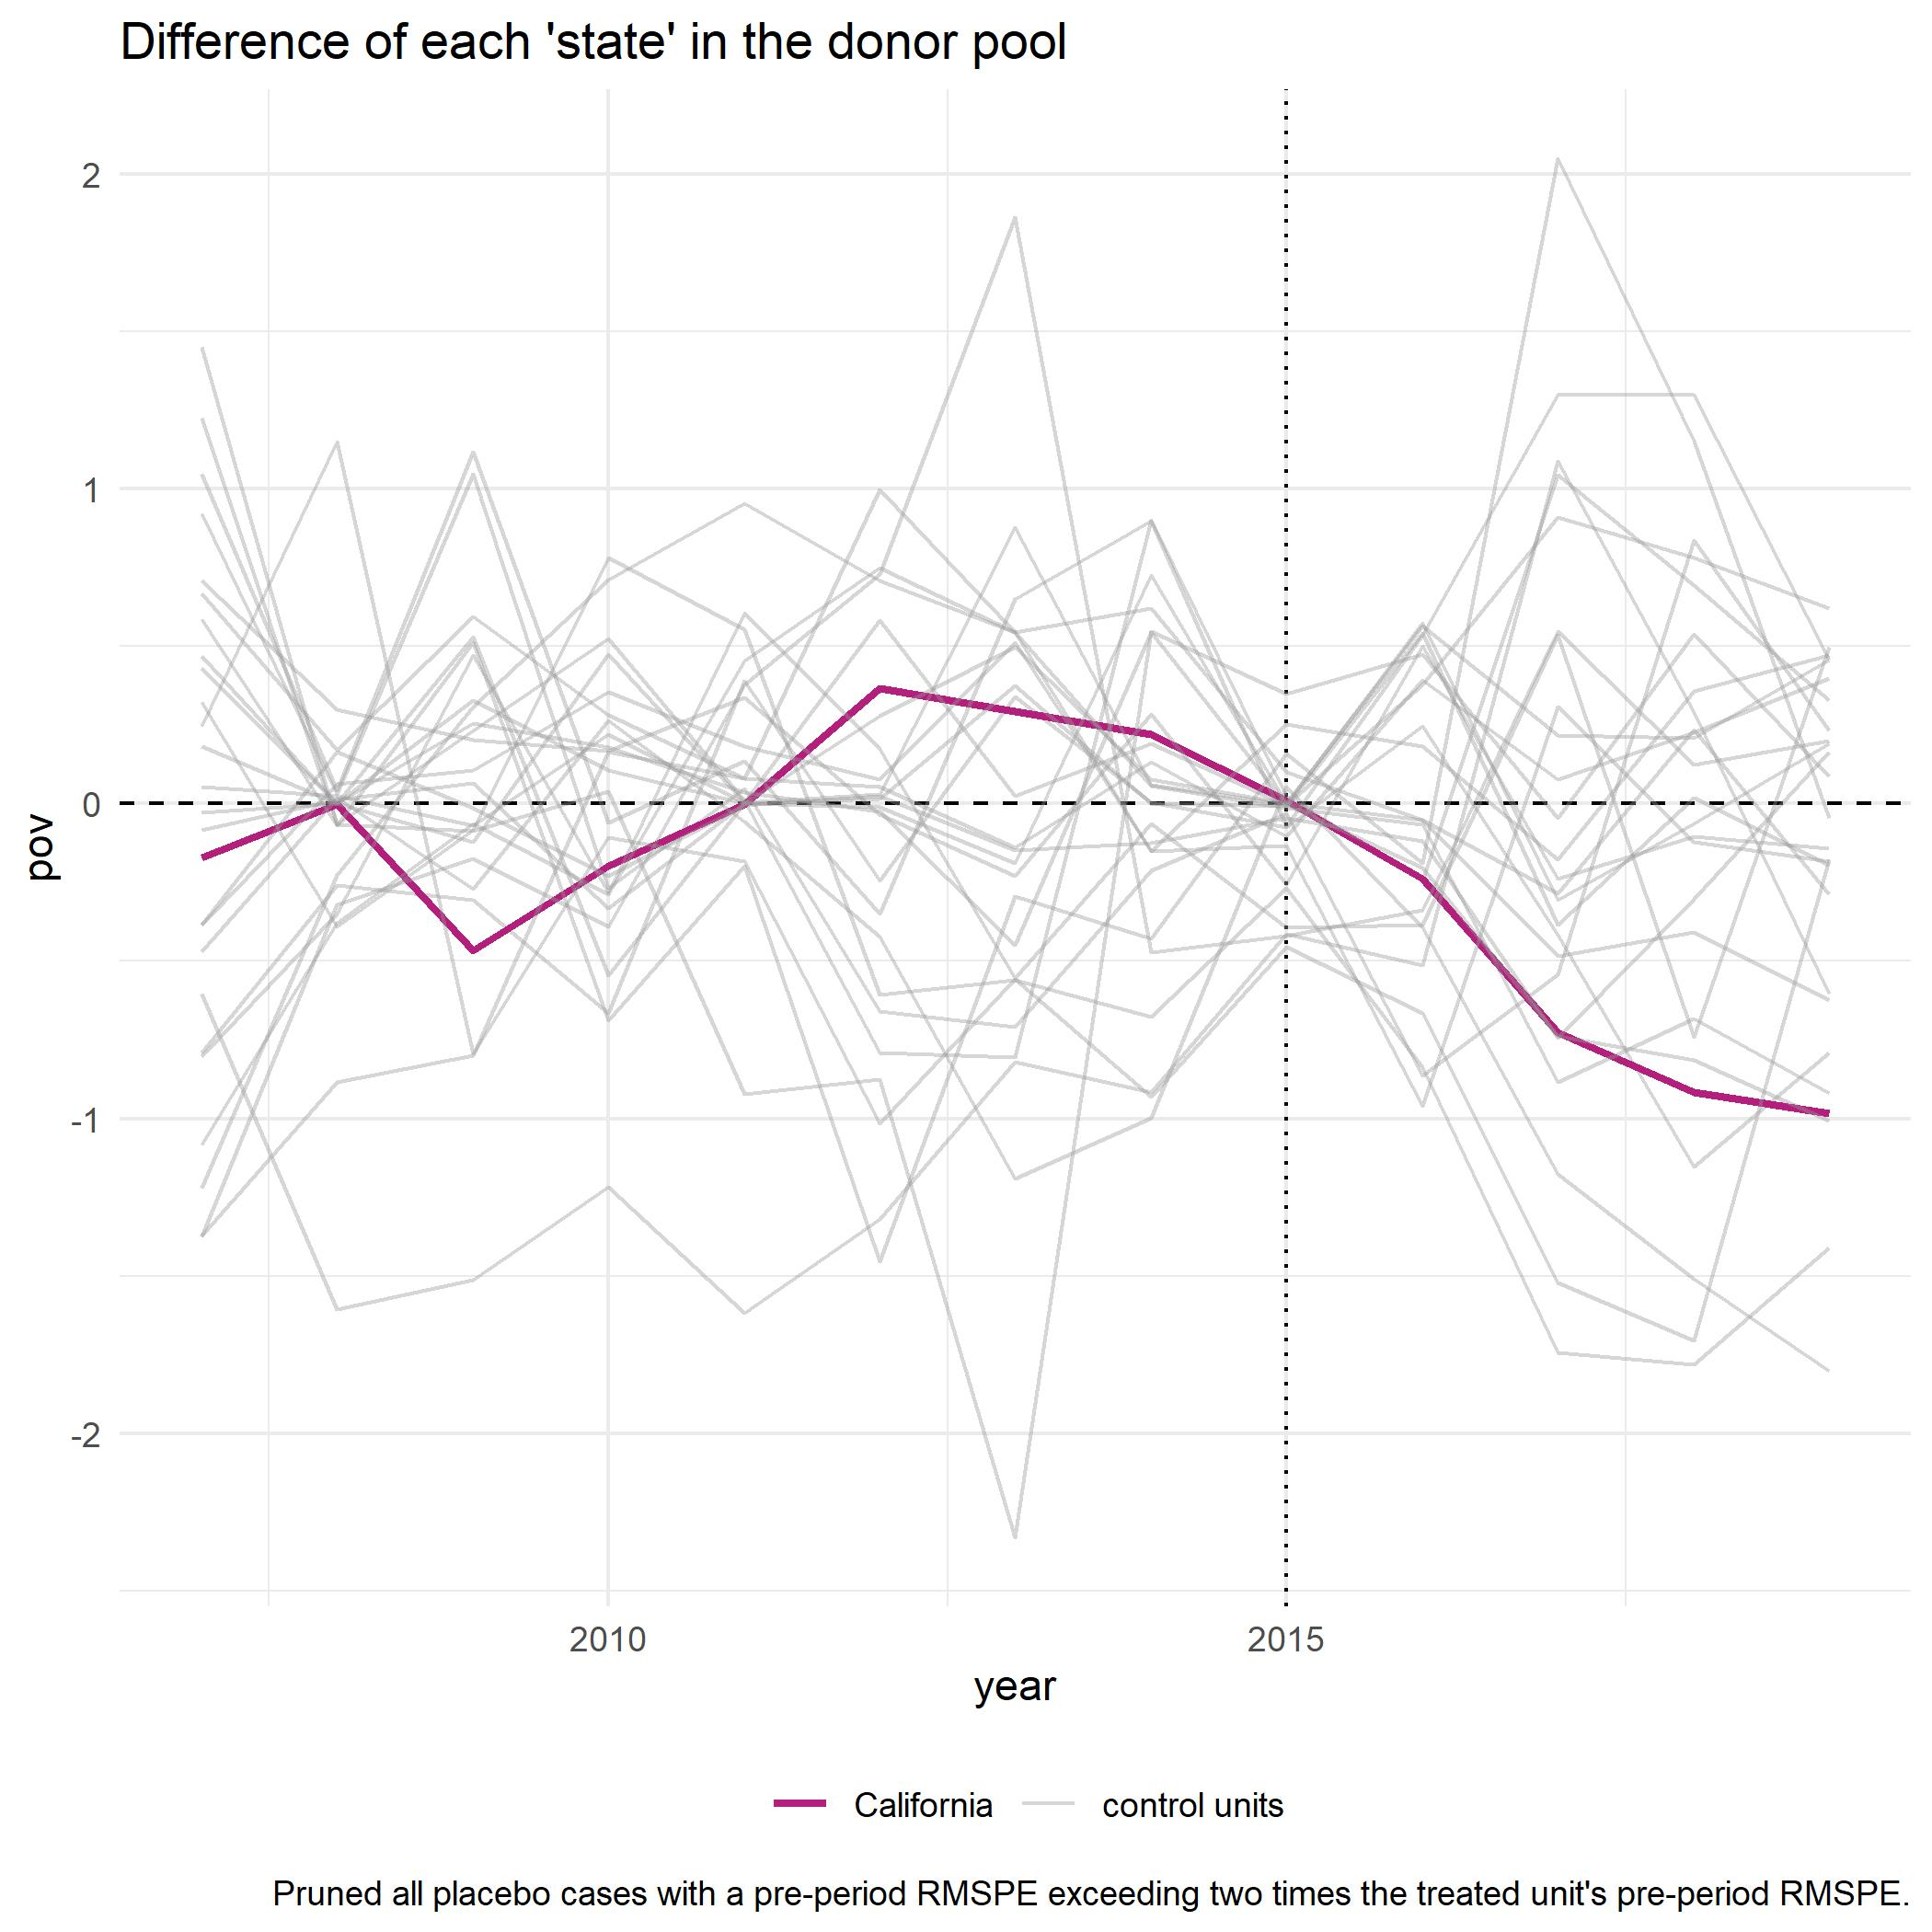
\includegraphics[width=.85\textwidth]{ca_pov_placebos}
    \end{center}
    \label{fig:ca_pov_placebos}{}
\end{figure}

Beginning with our poverty rate models, Figure~\ref{fig:ca_pov_placebos} shows some evidence in a decrease in the poverty rate. To determine a causal effect from a plot like this, we would hope to see the state's difference trend close to zero in the pre-treatment period, and then move along the outer margin of the other placebos. While there is some decrease in poverty following the treatment, it would be difficult to claim that the post-treatment trend is significantly lower than the placebos. There is some evidence about CalEITC's impact on the poverty rate in California, but it is hard to state conclusively that the EITC caused a reduction in poverty rates. 

For North Carolina, seen in Figure~\ref{fig:nc_pov_placebos}, the results are even more underwhelming. Although we fit our synthetic model well enough in the pre-treatment period, the post-treatment trend compared to placebos indicates that the effect of a decrease in poverty rates following elimination of the EITC in North Carolina could be produced by random chance. Therefore, we cannot confidently tease out a causal effect of removing the EITC policy on poverty rates in North Carolina. 

\begin{figure}[H]
    \caption{Poverty Gap in North Carolina and Poverty Placebo Gaps}
    \begin{center}
        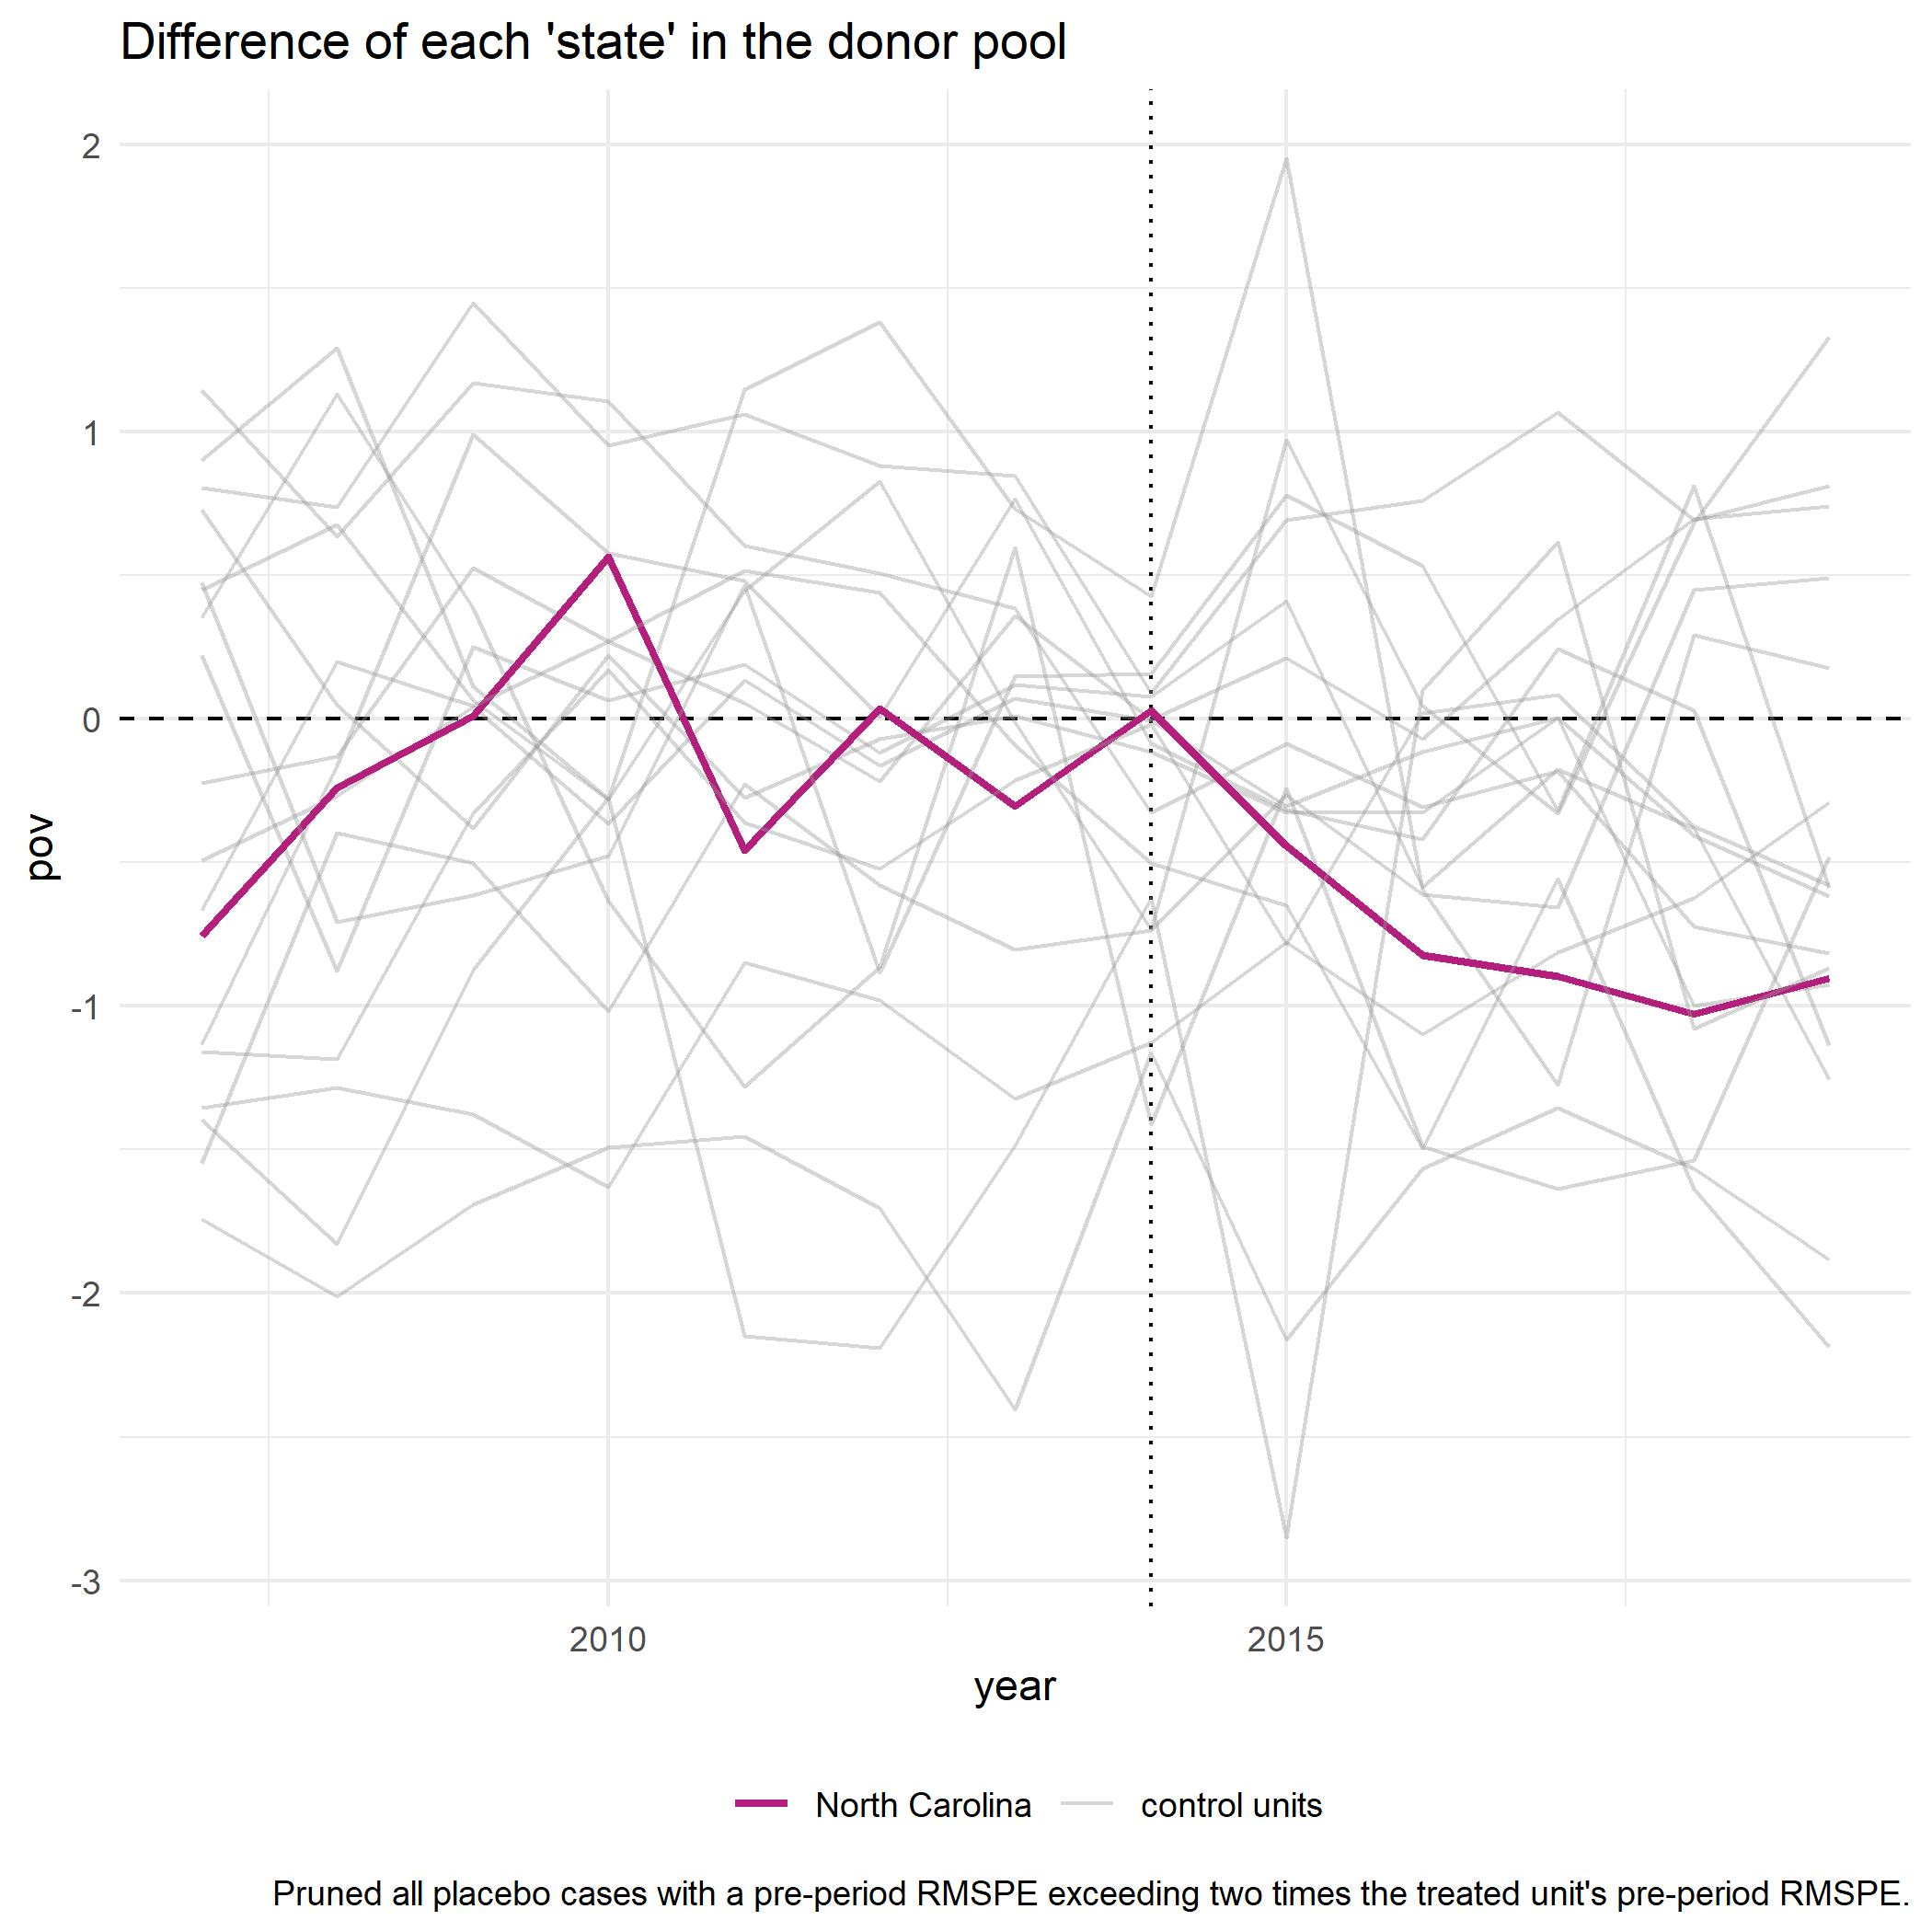
\includegraphics[width=.85\textwidth]{nc_pov_placebos}
    \end{center}
    \label{fig:nc_pov_placebos}{}
\end{figure}

Returning to labor force participation, where we previously saw some evidence of a positive relationship with the EITC, we apply the same iterative process to the states in the control groups to generate our placebos. These results are shown in Figures~\ref{fig:ca_lab_placebos} and~\ref{fig:nc_lab_placebos}. Similar to the case of our poverty models, our pre-treatment fit of the synthetic control is quite good, as evidenced by the state differenced trend hovering around zero. For both states, the superimposed purple line indicates a deviation from the control units after treatment against the convex hull of control units. North Carolina in particular is unusual in the donor pool, indicating that labor force participation was decreasing while the majority of the control units saw increases in the gap. Economic theory would suggest this relationship, but the results are still surprising given how modest the EITC was in North Carolina before it was eliminated. Notice that for these models, we pruned the population of placebos by removing states whose fit was more than two times the root mean-squared error of California and North Carolina, a cutoff that is considered highly restrictive, and provides strong evidence that we would not see this outcome by chance.

 \begin{figure}[H]
    \caption{Poverty Gap in North Carolina and Poverty Placebo Gaps}
    \begin{center}
        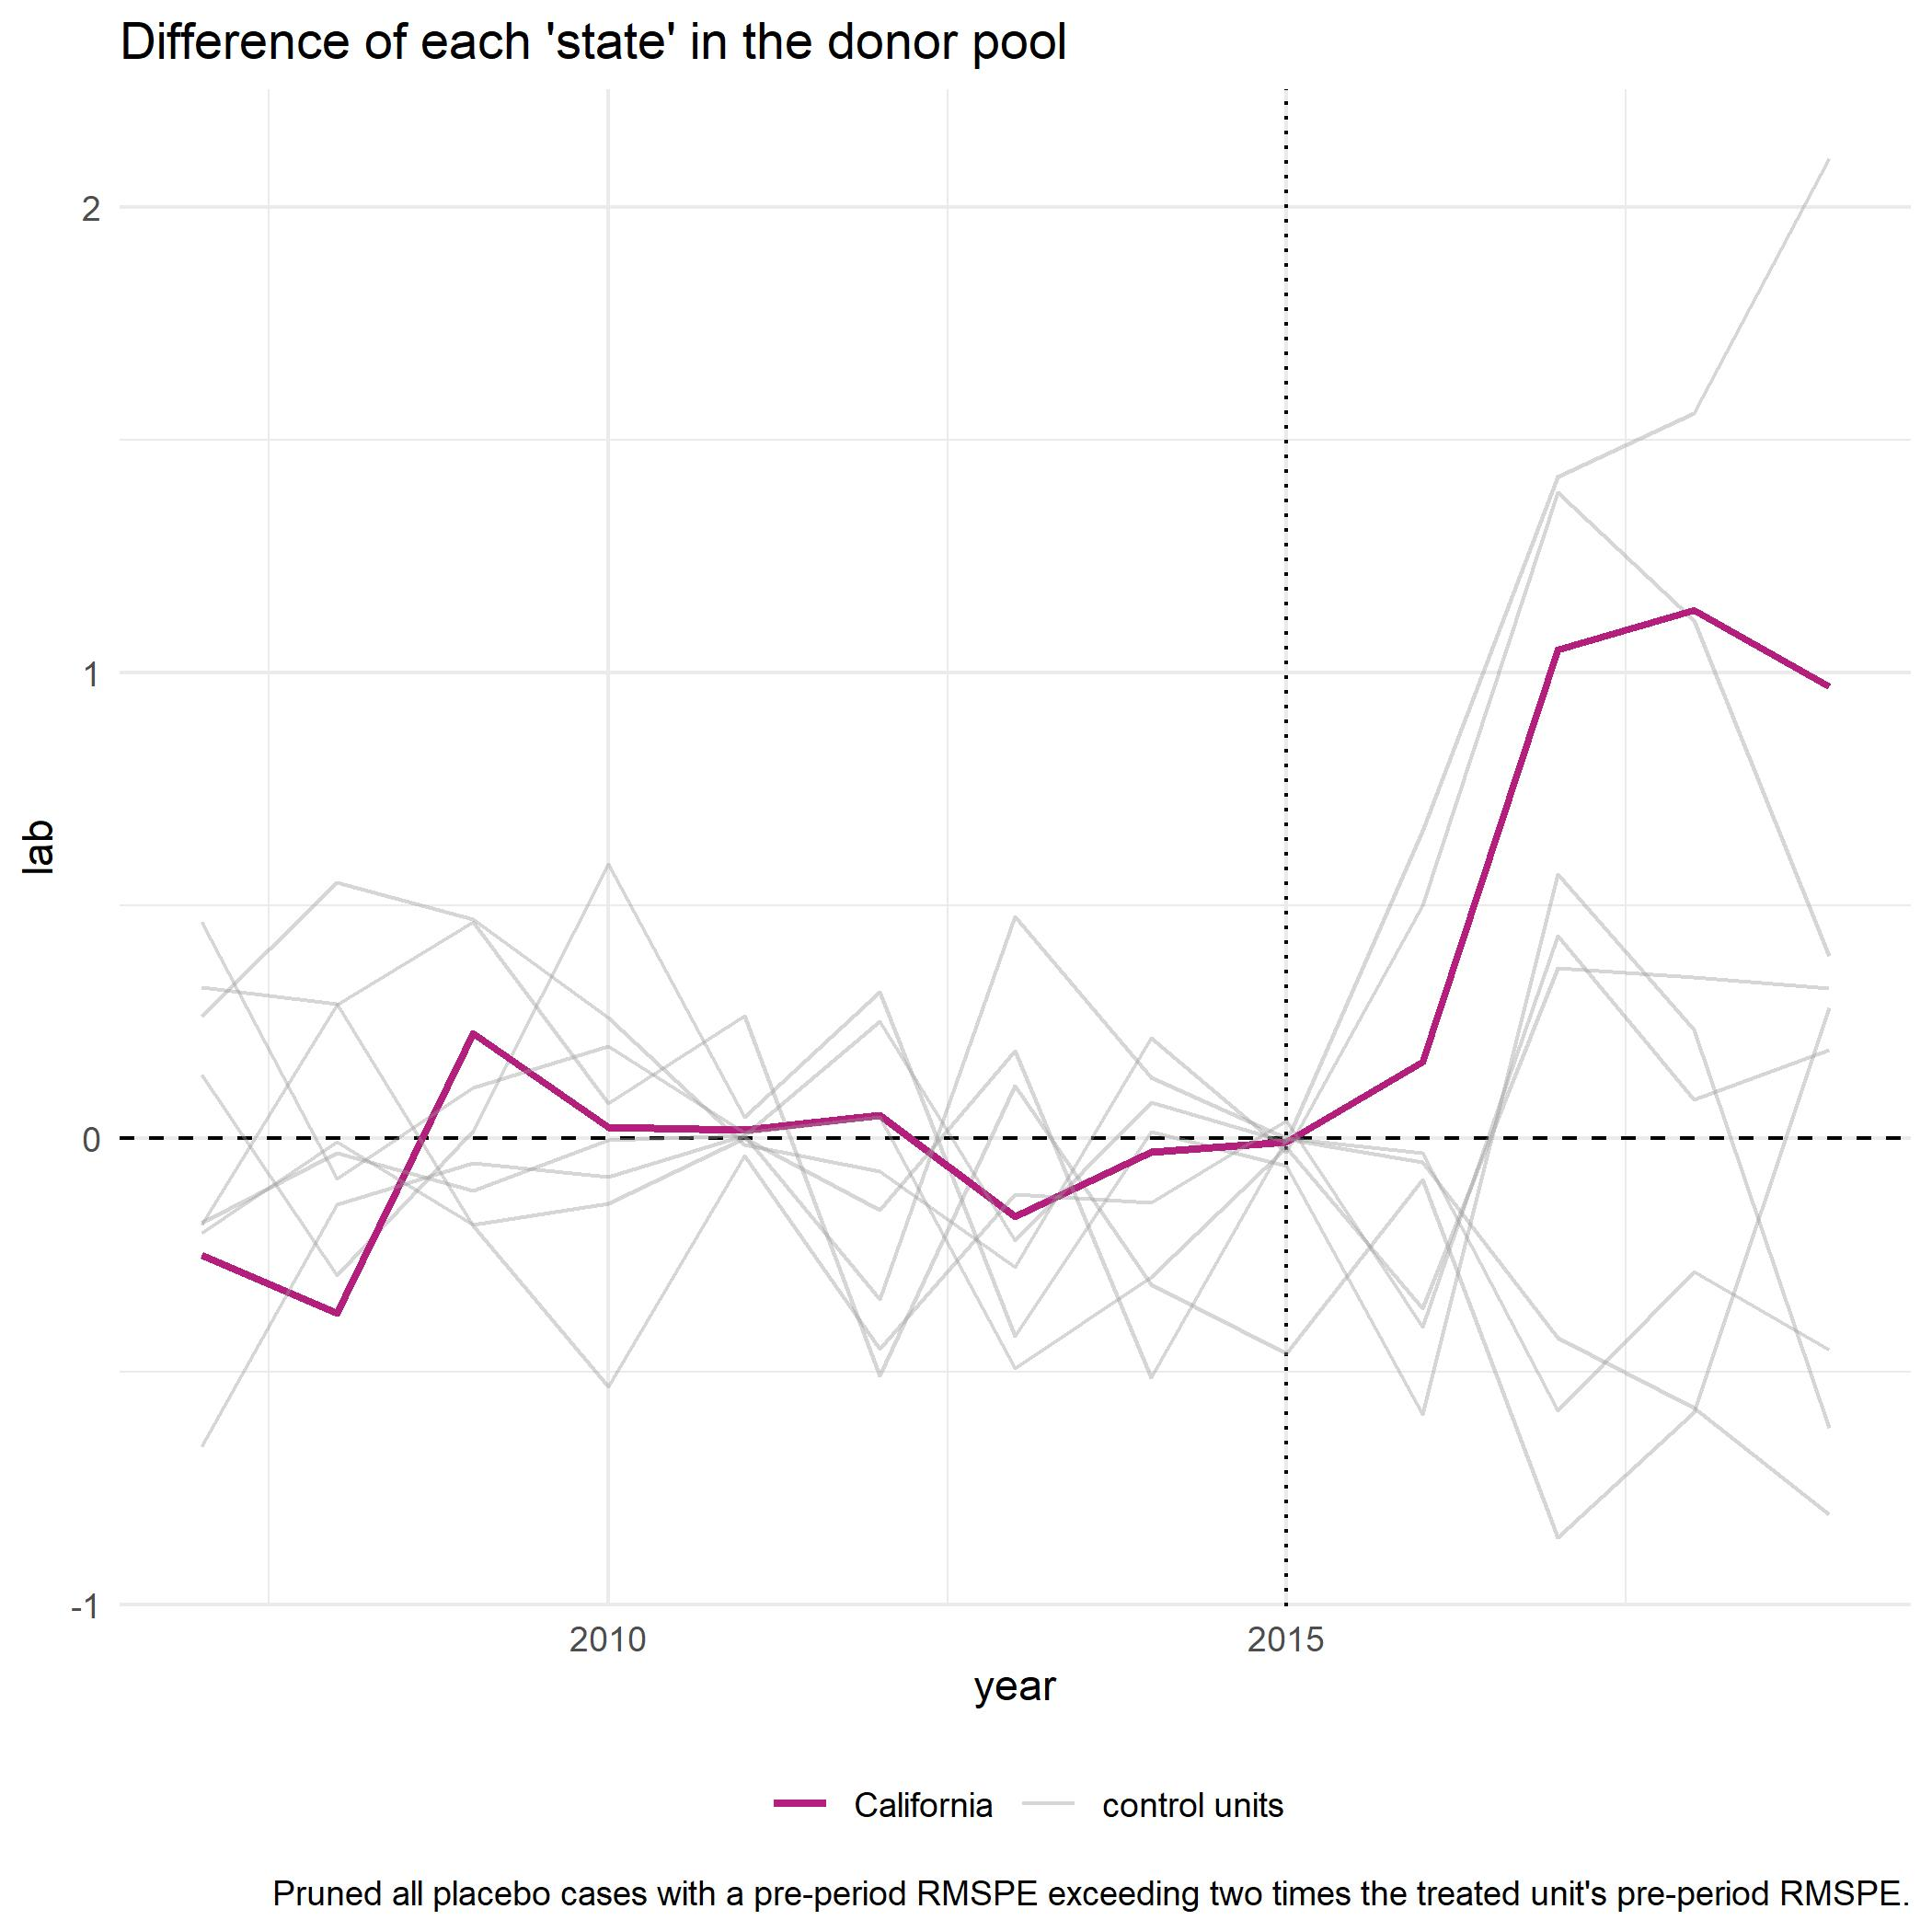
\includegraphics[width=.85\textwidth]{ca_lab_placebos}
    \end{center}
    \label{fig:ca_lab_placebos}{}
\end{figure}

 \begin{figure}[H]
    \caption{Labor Force Participation Gap in North Carolina and Labor Force Participation Placebo Gaps}
    \begin{center}
        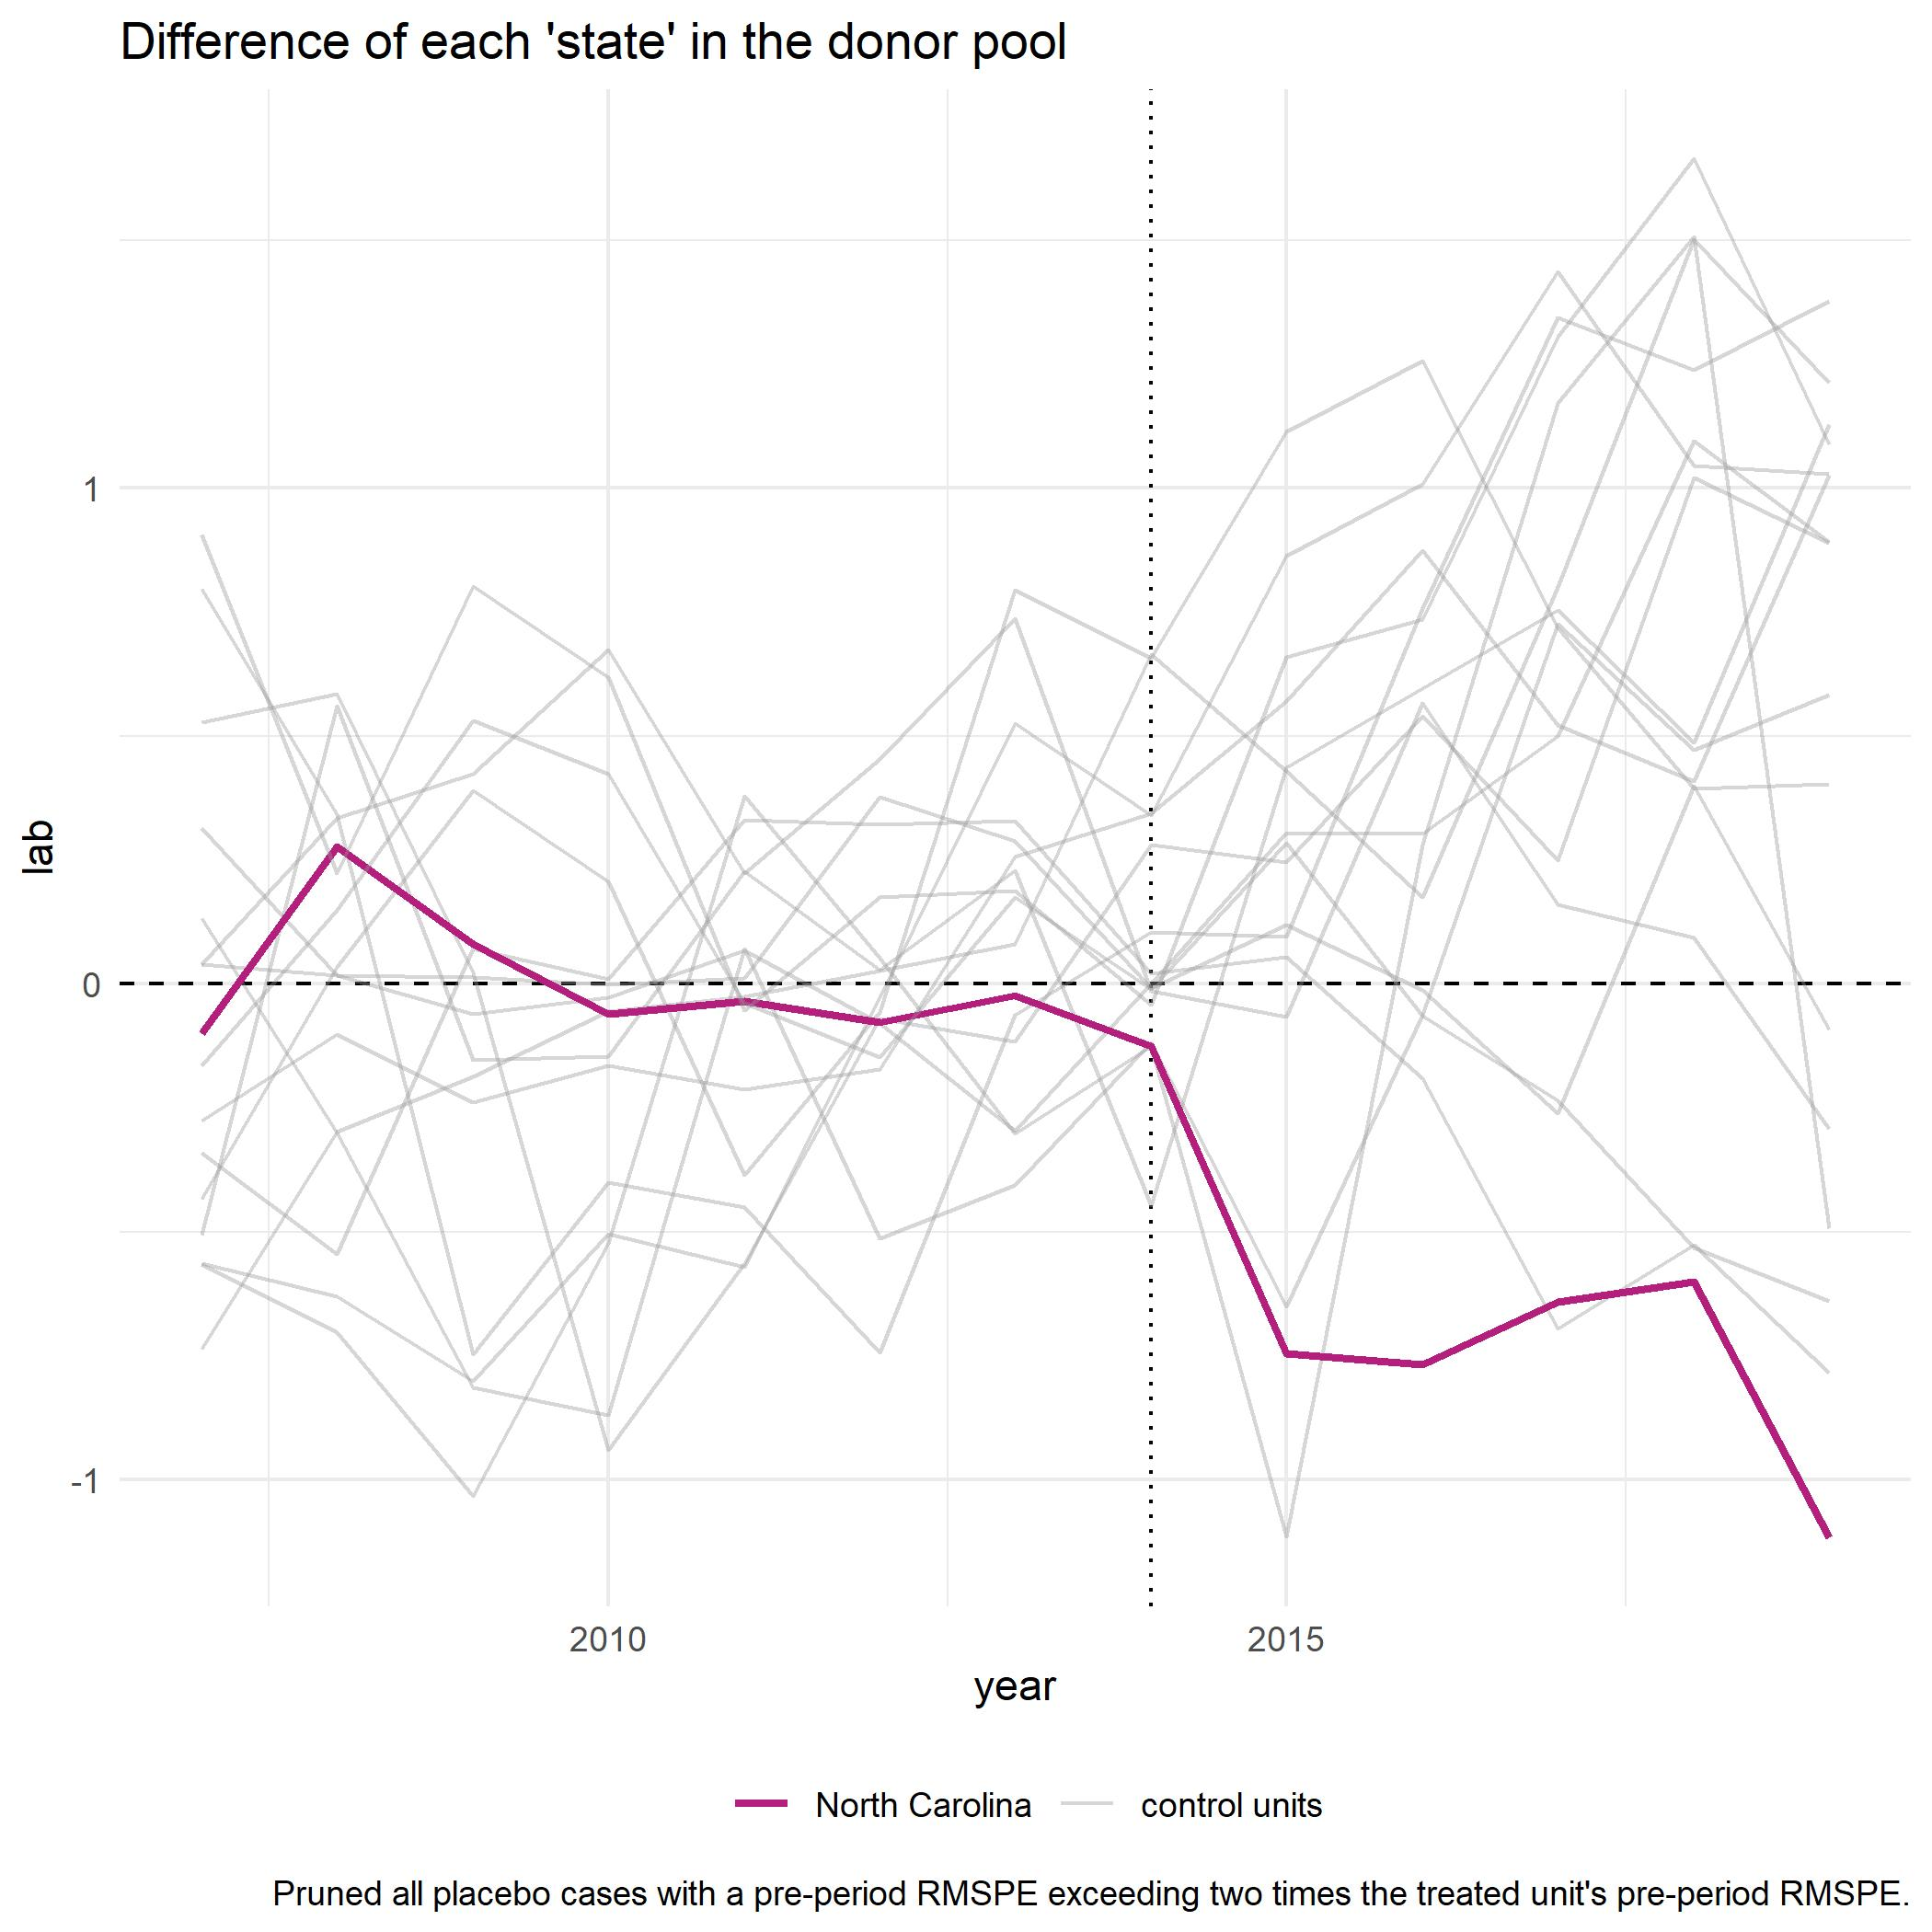
\includegraphics[width=.85\textwidth]{nc_lab_placebos}
    \end{center}
    \label{fig:nc_lab_placebos}{}
\end{figure}

\section{Conclusion}

The changes in state EITC policies in California and North Carolina provide us unique insight into the effect of Earned Income Tax Credits on labor force participation and poverty rates. We found evidence of an increase in the labor supply when an EITC is introduced in California, and a reduction in labor when the EITC is eliminated in North Carolina. We found signficantly less evidence of any change in the poverty rate in those states following the EITC changes. 

There are some important limitations and comments that need to be raised following our analysis. First, just because the policies did not have an appreciable effect on poverty in our results does not imply that the policy is misguided or useless. On the contrary, the refundable tax credits offered by way of the EITC represent real dollars in the hands of working families. Second, our results where limited somewhat by the data. A few more years of data will likely provide more clarity on the impact of the policy over time. We also did not have access to data that allowed us to explore poverty rates at the margins, and we could only evaluate the poverty rate as a whole. A more targeted exploration of households at or near the poverty level would allow for more conclusive results, and analysis segmented by household type (single parent, number of children, etc.) would provide further insight. As more states consider expanding their EITCs and policymakers at the federal level continue to use the EITC as a primary anti-poverty tool, continued study of the policy will be essential. 

With how important comparative case studies are in policy analysis, especially when there exists just one unit undergoing treatment, we found the process of applying weights to counterfactual control units and the exploratory units both enightening and challenging, especially with regard to choosing outcome variable lags. Given that \cite{athey2017state} called synthetic control ``arguably the most important innovation in the policy evaluation literature in the last 15 years," the changes in state EITC laws gave us good practical experience with the technique, and we plan to keep synthetic control in our arsenal of causal techniques into the future.  

\bibliography{bib}{}
\bibliographystyle{apalike}

\newpage
\section*{Appendix}

\InputTable{summarystats}
\InputTable{ca_lab}
\InputTable{ca_pov}
\InputTable{nc_lab}
\InputTable{nc_pov}



\end{document}
